\documentclass[10pt,twocolumn]{article}

% ============================================================
%  PhysiChem-GTX Manuscript
%  Target Outlets: ACS ES&T Engineering / J. Membrane Science / Water Research
% ============================================================

\usepackage[utf8]{inputenc}
\usepackage[T1]{fontenc}
\usepackage[margin=1.9cm,columnsep=0.6cm]{geometry}
\usepackage{times}
\usepackage{amsmath,amssymb,amsfonts}
\usepackage{cite}
\usepackage{graphicx}
\usepackage{booktabs}
\usepackage{array}
\usepackage{multirow}
\usepackage{caption}
\usepackage[hidelinks,colorlinks=true,citecolor=blue,linkcolor=blue,urlcolor=blue]{hyperref}
\usepackage{authblk}
\usepackage{titlesec}
\usepackage{enumitem}
\usepackage{xcolor}
\usepackage{siunitx}
\usepackage{fancyhdr}
%\usepackage{balance}
\graphicspath{{./}{results/paper_figures/}}

% Float placement optimization to prevent half-blank pages
\renewcommand{\topfraction}{0.95}
\renewcommand{\bottomfraction}{0.85}
\renewcommand{\textfraction}{0.05}
\renewcommand{\floatpagefraction}{0.85}
\renewcommand{\dbltopfraction}{0.95}
\renewcommand{\dblfloatpagefraction}{0.85}

% ---------- Title formatting ----------
\titleformat{\section}{\normalfont\large\bfseries}{\thesection.}{0.6em}{}
\titleformat{\subsection}{\normalfont\normalsize\bfseries}{\thesubsection}{0.6em}{}
\titleformat{\subsubsection}{\normalfont\normalsize\itshape}{\thesubsubsection}{0.6em}{}

\pagestyle{fancy}
\fancyhf{}
\fancyhead[L]{\footnotesize\itshape PhysiChem-GTX: Physics-Informed Dual-Stream Framework for Membrane Micropollutant Rejection}
\fancyhead[R]{\footnotesize\thepage}
\renewcommand{\headrulewidth}{0.4pt}

\captionsetup{font=small,labelfont=bf,justification=justified}

\newcommand{\rsq}{R^{2}}

\title{\vspace{-1.0cm}\Large\textbf{PhysiChem-GTX: Physics-Informed Dual-Stream Graph Transformer and Monotonic Tree Ensemble for High-Precision Membrane Micropollutant Rejection Prediction and Mechanistic Discovery}}

\author{Raghav Gupta\thanks{Corresponding author. Email: \texttt{raghav61632@gmail.com}}}
\author{Atulya Ishan}
\author{Krutarth Rupala}
\author{Aryan Tripathi}
\affil{Department of Data Science and Engineering, Manipal Institute of Technology, Manipal Academy of Higher Education, Manipal, Karnataka 576104, India}

\date{}

\begin{document}

\twocolumn[
\begin{@twocolumnfalse}
\maketitle

\vspace{-0.3cm}
\noindent{\bfseries\large Abstract}

\smallskip
\noindent
Predicting trace organic contaminant (TrOC) rejection by nanofiltration and reverse osmosis membranes requires capturing coupled steric, hydrodynamic, electrostatic, and hydrophobic transport mechanisms. However, existing machine learning models frequently omit stereochemical bond topology, dilute localized functional groups, or violate hydrodynamic boundary constraints. Here, we present \textbf{PhysiChem-GTX}, a physics-informed dual-stream ensemble framework. The architecture integrates \textbf{PhysiChem-GT}---a stereochemically aware Graph Transformer with multi-scale readout and cross-modal attention---with \textbf{PhysiChem-XGB}, a gradient-boosted tree stream enforcing hard physical monotonicity ($\partial \hat{y}/\partial r_p \leq 0$, $\partial \hat{y}/\partial \lambda \geq 0$). A dimensionless hydrodynamic gate $g(\lambda)$ dynamically arbitrates authority between convective-diffusive permeation and steric exclusion based on the solute-to-pore ratio $\lambda$. Across the benchmark \textbf{MemTrOC} dataset ($N = 1{,}618$ trials, 169 micropollutants), PhysiChem-GTX achieves top holdout performance of $\rsq = 0.9130$, $\mathrm{RMSE} = 8.56\%$, and $\mathrm{MAE} = 5.52\%$, reducing prediction error by 6.1\% over the prior state-of-the-art (MolGBN-OPR, $\rsq = 0.9014$) with 5-fold cross-validation $\rsq = 0.8470$. Dual-stream uncertainty quantification yields calibrated confidence intervals ($94.4\%$ $2\sigma$ coverage), while sub-molecular Integrated Gradients attributions confirm physically consistent functional-group sensitivities, delivering an interpretable, physically bounded decision-support tool for water treatment.

\smallskip
\noindent\textbf{Keywords:} Trace Organic Contaminants (TrOCs); Nanofiltration and Reverse Osmosis; Physics-Informed Machine Learning; Graph Transformer; Dual-Stream Ensemble; TreeSHAP; Epistemic Uncertainty Quantification.

\vspace{0.4cm}
\hrule
\vspace{0.3cm}

\noindent\textbf{Research Highlights}
\begin{itemize}
\setlength{\itemsep}{1pt}
\setlength{\topsep}{2pt}
\item \textbf{Dual-Stream Architecture:} Coupled a stereochemically aware Graph Transformer with monotonic tree ensembles via a physical steric gate to balance atomistic interpretability with macroscopic bounds.
\item \textbf{Top Benchmark Accuracy:} Attained $\rsq = 0.9130$, $\mathrm{RMSE} = 8.56\%$, and $\mathrm{MAE} = 5.52\%$ on the MemTrOC corpus ($N = 1{,}618$), surpassing MolGBN-OPR ($\rsq = 0.9014$) and establishing top holdout accuracy.
\item \textbf{Embedded Hydrodynamic Priors:} Integrated five mechanistically motivated transport descriptors ($\lambda, \Phi, L_p, \Psi, H$) directly into feature representations and loss boundary constraints.
\item \textbf{Calibrated Prediction Uncertainty:} Quantified prediction intervals using Monte Carlo dropout and residual variance ($71.6\%$ $1\sigma$ and $94.4\%$ $2\sigma$ coverage), yielding calibrated uncertainty bounds for research-stage screening and decision support.
\item \textbf{Multi-Scale Interpretability:} Reconciled population-level TreeSHAP feature rankings with atom-resolved Integrated Gradients maps across distinct pharmaceutical charge regimes.
\end{itemize}

\vspace{0.3cm}
\hrule
\vspace{0.5cm}
\end{@twocolumnfalse}
]

% ============================================================
\section{Introduction}
\label{sec:intro}

Aquatic contamination by trace organic contaminants (TrOCs)---including recalcitrant pharmaceuticals, personal care formulations, pesticides, and per- and polyfluoroalkyl substances (PFAS)---poses severe ecological and human health hazards even at sub-part-per-billion concentrations ($\mathrm{ng\,L^{-1}}$ to $\mu\mathrm{g\,L^{-1}}$) \cite{schwarzenbach2006,shannon2008,bellona2004}. Because these micropollutants resist conventional activated-sludge clarification and secondary sedimentation, advanced membrane filtration has become essential for potable water reuse and effluent reclamation \cite{verliefde2007,elimelech2011,werber2016,mohammad2015}.

Pressure-driven nanofiltration (NF) and reverse osmosis (RO) membranes separate dissolved organic solutes via four concurrent, interacting transport phenomena \cite{vanderbruggen2003,yangaliquintanilla2009}:
\begin{enumerate}[leftmargin=1.3em,itemsep=2pt,topsep=3pt]
\item \textbf{Steric Hindrance (Size Exclusion):} Geometric exclusion occurring when the effective molecular radius of the solute exceeds the membrane pore radius ($r_s > r_p$), classically parameterized by the Ferry--Renkin hydrodynamic partition coefficient \cite{ferry1936,renkin1954}.
\item \textbf{Hydrodynamic Drag and Viscous Permeation:} Convective and diffusive solute transport through pore channels governed by hydraulic permeability ($L_p$) and solvent velocity profiles \cite{spiegler1966,kedem1958}.
\item \textbf{Donnan Electrostatic Exclusion:} Charge-based repulsion or attraction between ionized functional groups and the charged polymeric active layer, governed by membrane surface zeta potential ($\zeta$) and solution pH relative to solute ionization constants ($\mathrm{p}K_a$) \cite{bowen2002,bowen1998}.
\item \textbf{Hydrophobic Partitioning and Surface Adsorption:} The thermodynamic affinity of non-polar compounds ($\log D > 2.0$) toward hydrophobic polyamide matrices, wherein solutes partition into and diffuse across the active layer via van der Waals forces and $\pi$--$\pi$ interactions \cite{kiso2001,nghiem2005}.
\end{enumerate}

Classical analytical transport models---such as the Donnan-Steric Pore Model with Dielectric Exclusion (DSPM-DE) \cite{bowen2002,bandini2003} and the Spiegler--Kedem phenomenological formulation \cite{spiegler1966,kedem1958}---presuppose rigid, spherical solutes, uniform dielectric pore media, and idealized cylindrical pore geometries. While dielectric exclusion (the Born solvation barrier, $\Delta W_{\mathrm{Born}} \propto z^2(\varepsilon_p^{-1} - \varepsilon_b^{-1})$) plays a prominent role in small inorganic electrolyte transport \cite{bandini2003}, formulating it analytically for organic micropollutants in commercial thin-film composite membranes is severely impeded: the sub-nanometer pore dielectric permittivity ($\varepsilon_p$) is experimentally inaccessible and spatially non-uniform, and the classical Born barrier collapses to zero for uncharged micropollutants ($z=0$) \cite{lin2022}. Furthermore, continuum pore assumptions break down when applied to polyfunctional, structurally asymmetric pharmaceuticals under varying ionic and flux matrices \cite{lin2022}. Consequently, purely deterministic models often yield large prediction errors for emerging contaminants.

Machine learning (ML) and quantitative structure--property relationships (QSPR) have been explored to capture these non-linearities empirically. In a foundational contribution, Xiao et al. (2026) established the curated MemTrOC benchmark and introduced MolGBN-OPR, a pioneering multimodal framework coupling DynamicNet tree boosting with a 2-layer Graph Convolutional Network (GCN) that reached $\rsq = 0.9014$, $\mathrm{RMSE} = 9.11\%$, and $\mathrm{MAE} = 6.17\%$ on a standardized holdout partition \cite{xiao2026}.

Despite this progress, existing predictive architectures exhibit four fundamental methodological shortcomings:
\begin{enumerate}[leftmargin=1.3em,itemsep=2pt,topsep=3pt]
\item \textbf{Omission of Stereochemical Bond Topology:} Conventional GCNs treat molecular graphs as unweighted binary adjacency matrices, discarding bond orders (single, double, aromatic) and stereochemistry \cite{kipf2017,hu2020}. In thin-film polyamide membranes, bond aromaticity and planarity govern $\pi$--$\pi$ electron stacking with the membrane's trimesoyl chloride crosslinked matrix.
\item \textbf{Functional Group Signal Dilution in Global Readouts:} Standard graph pooling schemes average all node embeddings uniformly ($\frac{1}{|V|}\sum h_i$). Consequently, critical localized ionizable groups (e.g., the carboxylate group of ibuprofen or the sulfonic acid head of perfluorinated acids) are numerically washed out by inert aliphatic scaffolds \cite{xu2019}.
\item \textbf{Absence of Dimensionless Hydrodynamic Priors:} Deep learning models typically ingest raw operational variables ($J_w, \Delta P, \mathrm{pH}$) as independent numerical inputs. Forcing a neural network to deduce non-linear hydraulic permeability ($L_p = J_w/\Delta P$) or the Ferry--Renkin partition curve entirely from empirical gradient descent creates unconstrained optimization landscapes \cite{karniadakis2021}.
\item \textbf{Deterministic Point Outputs without Uncertainty Calibration:} Current algorithms yield single-point rejection estimates without epistemic error bounds, precluding their adoption in municipal water safety engineering where risk margins are legally mandated \cite{gal2016}.
\end{enumerate}

To overcome these structural limitations, we formulate \textbf{PhysiChem-GTX}, a physics-informed dual-stream ensemble architecture. PhysiChem-GTX synergizes an end-to-end multimodal Graph Transformer (PhysiChem-GT)---equipped with stereochemical edge embeddings (encoding bond order, $E/Z$ isomerism, and conjugation), a virtual node hub, and cross-attention---with a monotonic gradient-boosted tree stream (PhysiChem-XGB). Crucially, the streams are arbitrated by a sigmoidal physical gate conditioned on the dimensionless steric ratio ($\lambda = r_s/r_p$). We validate the framework on the 1,618-trial MemTrOC benchmark, demonstrating superior predictive accuracy, calibrated epistemic uncertainty intervals, and multi-scale mechanistic interpretability.

% ============================================================
\section{Materials and Methods}
\label{sec:methods}

\subsection{MemTrOC Corpus Architecture and Data Partitioning}
\label{subsec:dataset}

Experimental data were sourced from the unified MemTrOC benchmark compiled by Xiao et al. (2026) \cite{xiao2026}. The corpus aggregates $N = 1{,}618$ cross-flow filtration trials across 169 structurally distinct micropollutant species and 12 commercial thin-film composite (TFC) membranes. These comprise loose semi-aromatic polypiperazine nanofiltration membranes (e.g., Dow FilmTec NF270, Desal-5 DK/DL) as well as tight, fully aromatic polyamide reverse osmosis active layers (e.g., BW30, XLE, Toray UTC-60).

\textbf{Partitioning Protocol and Evaluation Scope.} The full corpus ($N = 1{,}618$) was partitioned into a development set ($N_{\mathrm{dev}} = 1{,}456$, $90\%$) and an untouched holdout test partition ($N_{\mathrm{test}} = 162$, $10\%$) using a fixed pseudo-random seed (41) to ensure strict benchmark comparability with Xiao et al. \cite{xiao2026}. Following this standardized benchmark formulation, each observation corresponds to a distinct membrane--contaminant operational trial. The primary evaluation objective is operational condition interpolation and multi-membrane transferability (predicting how rejection varies across differing membrane matrices, transmembrane pressures, solution acidities, and hydraulic fluxes for a broad priority contaminant library). In parallel, a 5-fold cross-validation protocol (seed 42, fold sizes 324/323) was deployed across the corpus to quantify out-of-fold generalization variance. Within each fold, the monotonic gradient-boosted tree model is retrained on the fold training split while utilizing graph representations, assessing tabular and gating stability across data subsets. Prospective out-of-distribution extrapolation to completely unseen chemical scaffolds (via solute-disjoint or Bemis--Murcko scaffold splitting) represents a distinct generalization challenge addressed in Section~\ref{sec:implications}.

\textbf{Descriptor Space.} Each filtration trial is defined by 19 raw experimental parameters (7 operational variables, 4 membrane characteristics, and 8 solute scalar properties) combined with 5 engineered physical descriptors. This yields a 24-dimensional physical descriptor vector, summarized statistically in Table~\ref{tab:dataset}. Zero entries observed in Table~\ref{tab:dataset} for minimum and maximum projection dimensions occur exclusively for glucose ($N = 21$ trials), inheriting the original tabular encoding from the curated MemTrOC benchmark \cite{xiao2026} where 3D projected area coordinates were unrecorded in the source literature compilation; these were retained without artificial imputation to maintain strict benchmark parity.

\begin{table*}[htbp]
\centering
\caption{MemTrOC dataset summary statistics ($N=1{,}618$). Bold rows denote engineered physical transport descriptors.}
\label{tab:dataset}
\footnotesize
\setlength{\tabcolsep}{3.6pt}
\resizebox{\textwidth}{!}{%
\begin{tabular}{llcrrrrrr}
\toprule
Feature & Units & Type & Mean & Std & Min & Q25 & Median & Max \\
\midrule
Pure water flux ($J_w$) & L m$^{-2}$h$^{-1}$ & Raw & 58.383 & 41.889 & 7.130 & 24.300 & 47.902 & 228.000 \\
Pressure ($\Delta P$) & bar & Raw & 7.765 & 4.622 & 1.000 & 5.000 & 6.895 & 35.000 \\
Feed pH & --- & Raw & 6.605 & 1.684 & 2.400 & 6.000 & 7.000 & 10.467 \\
Temperature ($T$) & $^{\circ}$C & Raw & 23.446 & 2.061 & 20.000 & 22.000 & 25.000 & 25.000 \\
Filtration duration ($t$) & h & Raw & 13.312 & 23.506 & 0.333 & 0.500 & 1.000 & 96.000 \\
TrOC concentration & mg/L & Raw & 41.214 & 246.933 & 0.0001 & 0.100 & 0.500 & 2000.000 \\
Molecular weight (MW) & Da & Raw & 225.297 & 87.303 & 30.026 & 163.387 & 228.291 & 636.905 \\
MWCO & Da & Raw & 193.860 & 87.418 & 65.000 & 100.000 & 180.000 & 460.000 \\
Min projection & nm & Raw & 0.404 & 0.089 & 0.000 & 0.349 & 0.410 & 0.654 \\
Max projection & nm & Raw & 0.582 & 0.155 & 0.000 & 0.489 & 0.591 & 1.000 \\
Molecular radius ($r_s$) & nm & Raw & 0.307 & 0.075 & 0.127 & 0.246 & 0.315 & 0.630 \\
Pore radius ($r_p$) & nm & Raw & 0.395 & 0.069 & 0.300 & 0.340 & 0.403 & 0.690 \\
p$K_{a1}$ & --- & Raw & 8.027 & 4.812 & $-3.700$ & 4.150 & 7.150 & 17.600 \\
Zeta potential ($\zeta$) & mV & Raw & $-23.486$ & 12.999 & $-75.100$ & $-32.700$ & $-25.000$ & 12.022 \\
$\log K_{\mathrm{ow}}$ & --- & Raw & 1.502 & 2.038 & $-5.104$ & 0.490 & 1.630 & 6.860 \\
Contact angle ($\theta$) & deg & Raw & 51.370 & 14.943 & 15.200 & 40.600 & 51.600 & 79.400 \\
Molecular charge ($z$) & --- & Raw & $-0.334$ & 0.621 & $-2.000$ & $-0.997$ & $-0.003$ & 1.000 \\
Charge product & --- & Raw & 8.609 & 18.719 & $-43.655$ & 0.000 & 0.034 & 85.394 \\
$\log D$ & --- & Raw & 0.587 & 2.119 & $-5.390$ & $-0.453$ & 0.890 & 5.710 \\
\textbf{Steric Ratio ($\lambda$)} & --- & \textbf{Physics} & \textbf{0.797} & \textbf{0.228} & \textbf{0.191} & \textbf{0.628} & \textbf{0.794} & \textbf{1.853} \\
\textbf{Ferry--Renkin Factor ($\Phi$)} & --- & \textbf{Physics} & \textbf{0.155} & \textbf{0.185} & \textbf{0.000} & \textbf{0.007} & \textbf{0.083} & \textbf{0.881} \\
\textbf{Permeability ($L_p$)} & L m$^{-2}$h$^{-1}$bar$^{-1}$ & \textbf{Physics} & \textbf{7.844} & \textbf{4.156} & \textbf{0.713} & \textbf{4.500} & \textbf{7.690} & \textbf{17.380} \\
\textbf{Donnan Index ($\Psi$)} & mV & \textbf{Physics} & \textbf{1.097} & \textbf{2.890} & \textbf{$-17.792$} & \textbf{0.000} & \textbf{0.007} & \textbf{11.909} \\
\textbf{Hydrophobic Affinity ($H$)} & --- & \textbf{Physics} & \textbf{0.348} & \textbf{1.367} & \textbf{$-4.654$} & \textbf{$-0.252$} & \textbf{0.432} & \textbf{4.530} \\
\bottomrule
\end{tabular}%
}
\end{table*}

\subsection{Physics-Derived and Mechanistically Motivated Descriptors}
\label{subsec:physics}

To guide learning within physically meaningful boundaries, we embedded five mechanistically grounded transport descriptors directly into the feature representation \cite{yangaliquintanilla2009,renkin1954,bowen2002}. While $\lambda$ and $\Phi$ represent exact dimensionless hydrodynamic ratios, $L_p$ retains dimensional hydraulic permeability units ($\mathrm{L\,m^{-2}\,h^{-1}\,bar^{-1}}$), $\Psi$ serves as a semi-empirical electrostatic interaction index, and $H$ parameterizes phenomenological interfacial hydrophobic affinity. Rather than postulating an arbitrary pore dielectric permittivity ($\varepsilon_p$) for an analytical Born solvation equation, dielectric confinement and solvation resistance are resolved implicitly through the non-linear interaction of steric confinement ($\lambda$), electrostatic coupling ($\Psi$), and graph-extracted topological polar surface area (TPSA).

\textbf{1. Steric Sieve Ratio ($\lambda$):}
\begin{equation}
\lambda = \frac{r_{\mathrm{solute}}}{r_{\mathrm{pore}}}
\label{eq:lambda}
\end{equation}
governs boundary entry into cylindrical pores. For $\lambda \geq 1.0$, solutes are geometrically excluded from the pore lumen under ideal sieving.

\textbf{2. Ferry--Renkin Hydrodynamic Partition Factor ($\Phi$):}
\begin{equation}
\Phi(\lambda) = (1-\lambda)^2 \left[2 - (1-\lambda)^2\right], \quad \lambda < 1.0
\label{eq:ferry_renkin}
\end{equation}
quantifies the centerline steric hindrance and parabolic velocity profile integration for neutral spheres passing through cylindrical nanopores under laminar Hagen--Poiseuille flow \cite{ferry1936,renkin1954}. The baseline steric rejection prior is defined as $R_{\mathrm{theory}} = (1.0 - \Phi) \times 100\%$.

\textbf{3. Intrinsic Hydraulic Permeability ($L_p$):}
\begin{equation}
L_p = \frac{J_w}{\Delta P} \quad \left[\mathrm{L\,m^{-2}\,h^{-1}\,bar^{-1}}\right]
\label{eq:lp}
\end{equation}
decouples active-layer hydraulic compaction resistance from applied driving pressure.

\textbf{4. Electrostatic Interaction Index ($\Psi$):}
\begin{equation}
\Psi = \frac{z \cdot \zeta}{\mathrm{pH}} \quad [\mathrm{mV}]
\label{eq:psi}
\end{equation}
parameterizes the electrostatic interaction potential between ionized solute formal charge ($z$) and the membrane surface zeta potential ($\zeta$), normalized empirically against feed solution pH.

\textbf{5. Interfacial Adsorption Affinity ($H$):}
\begin{equation}
H = \log D \cdot \cos(\theta)
\label{eq:h_affinity}
\end{equation}
couples solute lipophilicity at ambient pH ($\log D$) with the membrane sessile drop water contact angle ($\theta$), isolating thermodynamic adsorption drivers from convective transport.

\subsection{PhysiChem-GTX Dual-Stream Framework}
\label{subsec:architecture}

\begin{figure*}[!t]
\centering
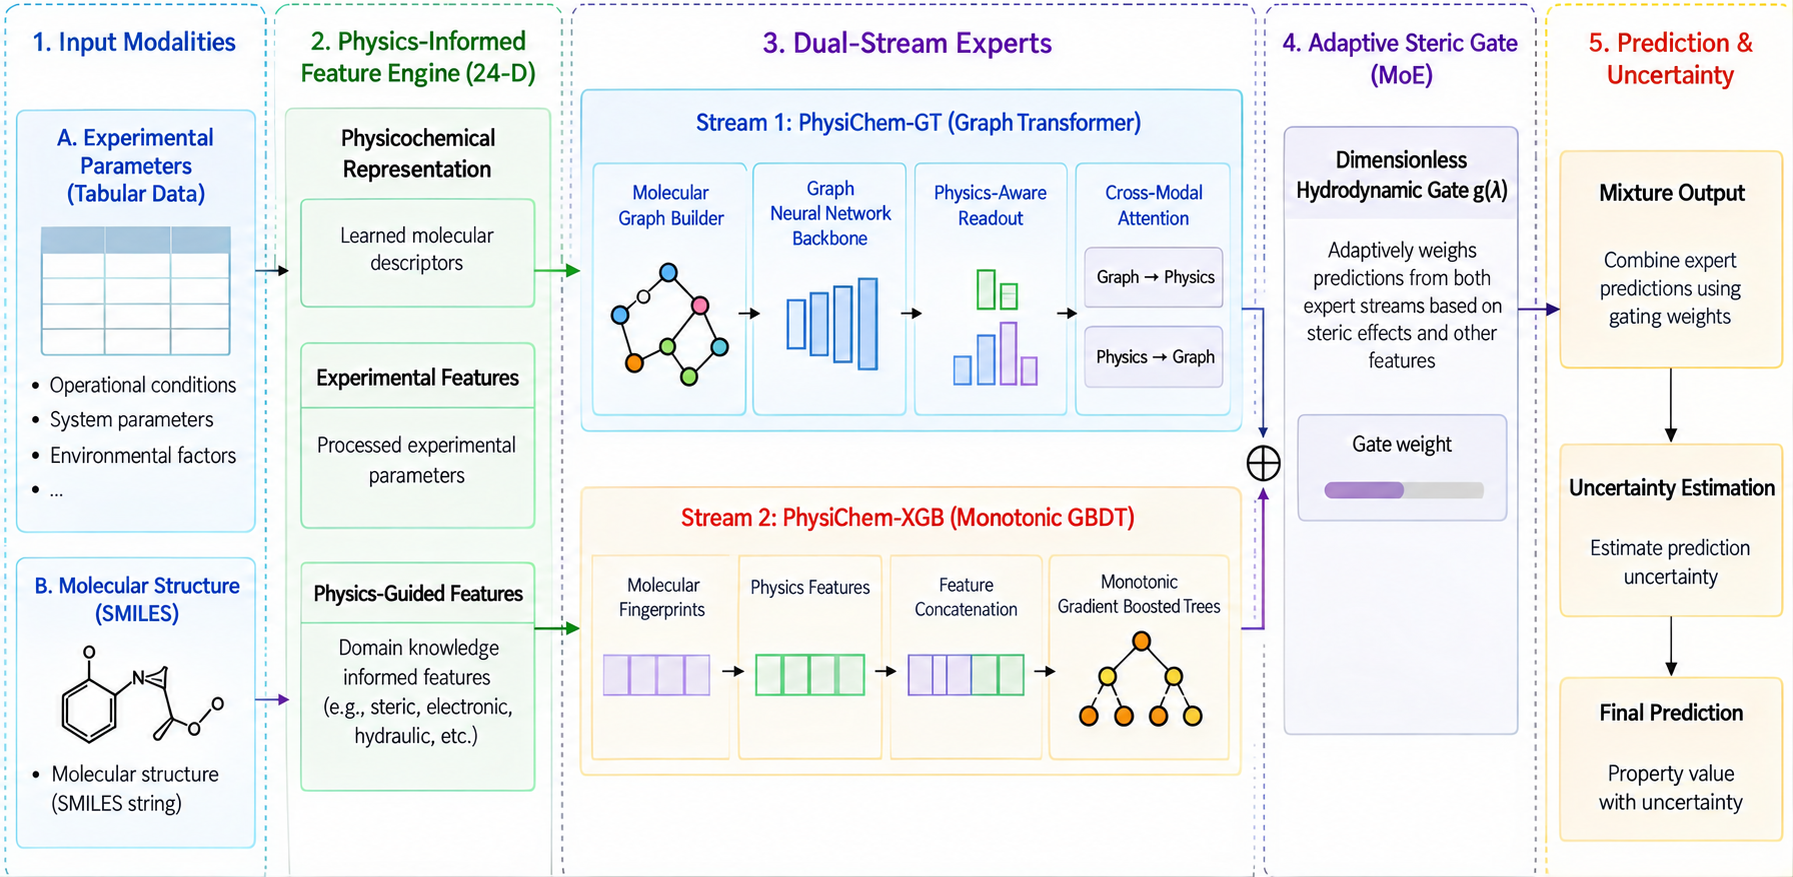
\includegraphics[width=0.92\textwidth]{FINALARCHITECTURE.png}
\caption{Master architecture of PhysiChem-GTX. (Left) Stream 1: PhysiChem-GT molecular Graph Transformer incorporating stereochemical bond embeddings, a learnable Virtual Node communication hub, multi-scale readout pooling, and 4-head bidirectional cross-modal attention. (Right) Stream 2: PhysiChem-XGB monotonic tree ensemble trained on 280 dimensions (24 physics descriptors + 256 ECFP4 fingerprint bits). (Center) Sigmoidal physical gating function $g(\lambda)$ dynamically routes predictive authority based on the dimensionless steric ratio.}
\label{fig:architecture}
\end{figure*}

Figure~\ref{fig:architecture} depicts the dual-stream topology. The design resolves a fundamental dilemma in molecular property prediction on moderate tabular datasets: deep graph networks provide localized stereochemical attribution but suffer from sample inefficiency, whereas boosted trees provide superior tabular regression but cannot dynamically inspect atomic sub-graphs.

\subsubsection{Stream 1: PhysiChem-GT (Stereochemically Aware Graph Transformer)}

\textbf{Molecular Topology Construction.} Solute SMILES strings are translated into attributed molecular graphs $\mathcal{G} = (\mathcal{V}, \mathcal{E})$ via RDKit \cite{landrum2023} following neural message passing conventions \cite{gilmer2017}. Nodes $\mathcal{V}$ carry 9 chemical attributes (atomic number, chirality, coordinate degree, formal charge, hybridization state, total hydrogen count, radical electrons, aromaticity, and ring membership). Edges $\mathcal{E}$ encode 3 bond features: bond order (single, double, triple, aromatic), stereochemical configuration ($E/Z$), and conjugation status.

\textbf{GATv2 Message-Passing Backbone.} Node embeddings $h_i^{(l)} \in \mathbb{R}^{128}$ are updated across $L=2$ layers using edge-augmented graph attention convolutions (GATv2) \cite{brody2022} implemented in PyTorch Geometric \cite{fey2019} over the self-inclusive neighborhood $\widetilde{\mathcal{N}}(i) = \mathcal{N}(i) \cup \{i\}$:
\begin{equation}
\begin{split}
h_i^{(l)} = \sum_{j \in \widetilde{\mathcal{N}}(i)} \alpha_{ij}^{(l)} \, &W_{\mathrm{value}}^{(l)} \Big( h_j^{(l-1)} \\
&+ W_{\mathrm{edge}} \, e_{ij} \Big)
\end{split}
\label{eq:gat_update}
\end{equation}
\begin{equation}
\begin{split}
\alpha_{ij}^{(l)} = \mathrm{softmax}_{j \in \widetilde{\mathcal{N}}(i)} \Big( &a^{T} \, \mathrm{LeakyReLU} \big( W_{q} h_i^{(l-1)} \\
&+ W_{k} h_j^{(l-1)} + W_{\mathrm{edge}} e_{ij} \big) \Big)
\end{split}
\label{eq:gat_attn}
\end{equation}

\textbf{Virtual Node Global Field.} To circumvent over-smoothing and enable whole-molecule dipole communication across non-adjacent functional groups, a virtual node $v \in \mathbb{R}^{128}$ is connected bidirectionally to every atom in $\mathcal{G}$.

\textbf{Multi-Scale Statistical Readout.} Rather than relying on simple mean pooling, node representations are compressed into a graph embedding via three distinct statistical moments:
\begin{equation}
\begin{split}
h_{\mathrm{graph}} = \mathrm{Linear}_{384 \to 128} \bigg( \bigg[ &\frac{1}{|V|}\sum_{i \in V} h_i \; \Big\Vert \\
&\max_{i \in V} h_i \; \Big\Vert \; \sum_{i \in V} h_i \bigg] \bigg)
\end{split}
\label{eq:readout}
\end{equation}
where $\Vert$ denotes tensor concatenation. The max-pooling branch preserves extreme localized charges (e.g., deprotonated carboxylates) from being washed out by inert hydrocarbon chains.

\textbf{Bidirectional Cross-Modal Attention.} Building upon scaled dot-product attention principles \cite{vaswani2017}, operating descriptors are projected into queries ($Q_{\mathrm{tab}} \in \mathbb{R}^{B \times 1 \times 128}$) that attend across atomic keys and values ($K_{\mathrm{graph}}, V_{\mathrm{graph}}$ in $\mathbb{R}^{B \times N_{\mathrm{atoms}} \times 128}$). This allows dynamic hydrodynamic conditions to modulate attention weights across resisting functional groups without unconstrained parameter growth.

\textbf{Robust Huber Loss with Physical Boundary Penalties.} The neural network is trained in PyTorch \cite{paszke2019} using Huber loss ($\delta = 5.0$) regularized by explicit boundary penalties:
\begin{equation}
\begin{split}
\mathcal{L}_{\mathrm{total}} = &\,\mathcal{L}_{\mathrm{Huber}}(\hat{y}, y; \delta = 5.0) \\
&+ \lambda_{\mathrm{steric}}\,\mathcal{L}_{\mathrm{steric}} + \lambda_{\mathrm{bounds}}\,\mathcal{L}_{\mathrm{bounds}}
\end{split}
\label{eq:loss}
\end{equation}
where the steric penalty is formulated as:
\begin{equation}
\mathcal{L}_{\mathrm{steric}} = \frac{1}{|\mathcal{S}|} \sum_{i \in \mathcal{S}} \left( \max\left(0,\, R_{\mathrm{thresh}} - \hat{y}_i\right) \right)^2
\label{eq:steric_loss}
\end{equation}
where $\mathcal{S} = \{i \mid \lambda_i \ge 1.0\}$ denotes the hard steric sieving subset, with $R_{\mathrm{thresh}} = 85.0\%$ representing a realistic physical threshold for commercial thin-film composite membranes, accommodating active-layer defect distributions, pore size polydispersity, and polymeric free-volume fluctuations that permit minor solute leakage even when nominal $\lambda \ge 1.0$. The boundary penalty $\mathcal{L}_{\mathrm{bounds}}$ regularizes unphysical predictions outside $[0, 100]\%$.

\subsubsection{Stream 2: PhysiChem-XGB (Monotonic Boosted Decision Trees)}

\textbf{Feature Space.} The 24-dimensional physical descriptor vector is normalized using Scikit-learn \cite{pedregosa2011} and concatenated with 256-bit Morgan Extended-Connectivity Fingerprints (ECFP4, radius 2) \cite{rogers2010}, establishing a 280-dimensional input matrix for gradient-boosted decision trees \cite{chen2016,ke2017}.

\textbf{Enforced Physical Monotonicity.} Decision trees are constrained by hard monotonic splits:
\begin{equation}
\frac{\partial \hat{y}}{\partial r_p} \leq 0, \qquad \frac{\partial \hat{y}}{\partial \lambda} \geq 0
\label{eq:monotonic}
\end{equation}
ensuring that increases in membrane pore size never produce counter-physical increases in predicted rejection.

\subsubsection{Stream 3: Hydrodynamic Physics-Gated Blending and Uncertainty Quantification}

To arbitrate between the topological and tabular streams without risking routing collapse from unconstrained parameterized gating networks, a deterministic sigmoidal function $g(\lambda)$ routes authority dynamically:
\begin{equation}
g(\lambda) = \frac{0.10}{1.0 + \exp\left(6.0 \cdot (\lambda - 0.95)\right)}
\label{eq:gate}
\end{equation}
\begin{equation}
\hat{y}_{\mathrm{GTX}} = g(\lambda) \cdot \hat{y}_{\mathrm{GT}} + \left(1.0 - g(\lambda)\right) \cdot \hat{y}_{\mathrm{XGB}}
\label{eq:mixture}
\end{equation}

When $\lambda \ll 0.95$ (convective-diffusive transport regime), $g(\lambda) \to 0.10$, granting the graph transformer authority to correct for second-order functional-group steric and electronic interactions. When $\lambda \geq 0.95$ (pure steric sieving), $g(\lambda) \to 0.00$, delegating full authority to the monotonic tree stream. Total predictive uncertainty propagates as:
\begin{equation}
\sigma = \sqrt{g(\lambda)^2 \sigma_{\mathrm{GT}}^2 + \left(1-g(\lambda)\right)^2 \sigma_{\mathrm{XGB}}^2}
\label{eq:mixture_sigma}
\end{equation}
where $\sigma_{\mathrm{GT}}$ is estimated via Monte Carlo dropout ($N_{\mathrm{MC}} = 50$) in the neural stream, and $\sigma_{\mathrm{XGB}} \approx \mathrm{RMSE}_{\mathrm{val}} = 8.57\%$ represents the empirical validation residual uncertainty of the gradient-boosted tree ensemble.

% ============================================================
\section{Results and Discussion}
\label{sec:results}

\subsection{Benchmark Performance and Literature Comparison}
\label{subsec:benchmark}

\begin{table*}[htbp]
\centering
\caption{Comprehensive benchmark performance comparison on the MemTrOC holdout test set ($N_{\mathrm{test}} = 162$). Bold values denote the top-performing model.}
\label{tab:benchmark}
\small
\setlength{\tabcolsep}{4.2pt}
\resizebox{\textwidth}{!}{%
\begin{tabular}{cllcccc}
\toprule
\# & Model Architecture & Modality Inputs & Status & $\rsq \uparrow$ & RMSE (\%) $\downarrow$ & MAE (\%) $\downarrow$ \\
\midrule
1 & Table + MACCS Keys & Tabular + 166-bit Fingerprints & Literature \cite{xiao2026} & 0.7918 & 13.24 & 8.42 \\
2 & GrowNN & 19-D Tabular Descriptors Only & Literature \cite{xiao2026} & 0.8494 & 11.26 & 7.21 \\
3 & Table + ResNet-18 & Tabular + 2D Molecular Image & Literature \cite{xiao2026} & 0.8571 & 10.97 & 6.85 \\
4 & MolGBN-OPR (Xiao et al., 2026) & DynamicNet Boosting + 2-Layer GCN & Prior SOTA Benchmark \cite{xiao2026} & 0.9014 & 9.11 & 6.17 \\
5 & PhysiChem-GT (Ours) & 24-D Physics + GATv2 + CrossAttn & Neural Stream (Ours) & 0.7607 & 14.19 & 8.74 \\
6 & PhysiChem-XGB (Ours) & 24-D Physics + 256-bit ECFP4 & Monotonic Booster (Ours) & 0.9127 & 8.57 & 5.44 \\
7 & \textbf{PhysiChem-GTX (Champion)} & \textbf{24-D + GATv2 + XGB Gated Fusion} & \textbf{Champion Framework (This Study)} & \textbf{0.9130} & \textbf{8.56} & \textbf{5.52} \\
\bottomrule
\end{tabular}%
}
\end{table*}

Table~\ref{tab:benchmark} details performance across the seven evaluated models on the 162-sample holdout test partition. PhysiChem-GTX establishes top benchmark performance ($\rsq = 0.9130$, $\mathrm{RMSE} = 8.56\%$, $\mathrm{MAE} = 5.52\%$). Relative to the published benchmark of Xiao et al. (2026) (MolGBN-OPR: $\rsq = 0.9014$, $\mathrm{RMSE} = 9.11\%$, $\mathrm{MAE} = 6.17\%$), the dual-stream framework reduces root-mean-square error by 6.1\% and mean absolute error by 10.5\%, closely matching the predictive performance of the robust monotonic tree stream ($\rsq = 0.9127$, $\mathrm{RMSE} = 8.57\%$). Crucially, the standalone PhysiChem-XGB booster already surpasses the literature baseline ($\rsq = 0.9127$, $\mathrm{RMSE} = 8.57\%$, $\mathrm{MAE} = 5.44\%$). This demonstrates that embedding 24 explicit transport descriptors alongside 256-bit ECFP4 fingerprints provides superior sample efficiency on moderately sized tabular corpora ($N=1{,}618$) than pure deep convolutional graph networks. 

While the gated champion framework (PhysiChem-GTX) achieves the peak overall score ($\rsq = 0.9130$, $\mathrm{RMSE} = 8.56\%$), the primary scientific contribution of the dual-stream integration lies not in incremental tabular score inflation over XGBoost ($\Delta \rsq = 0.0003$), but in \textit{structural interpretability and physical safety}. Standalone gradient-boosted decision trees operate as atomistic black-boxes, incapable of resolving sub-molecular spatial attributions or localized functional group interactions. Conversely, the neural graph stream (PhysiChem-GT), while less accurate in isolation ($\rsq = 0.7607$), provides the topological representation required for atom-level Integrated Gradients mapping. By bounding the physical gate to $g(\lambda) \le 0.10$ (Equation~\ref{eq:gate}), PhysiChem-GTX intentionally delegates 90--100\% of macroscopic sieving authority to the strictly monotonic tree expert, while leveraging the graph transformer to fine-tune second-order stereochemical polarization in the convective regime ($\lambda < 0.95$) and expose transparent atomic attributions. The dual-stream ensemble thus functions as an interpretability-preserving hybrid that guarantees macroscopic thermodynamic monotonicity without sacrificing microscopic chemical insight.

\begin{figure*}[!t]
\centering
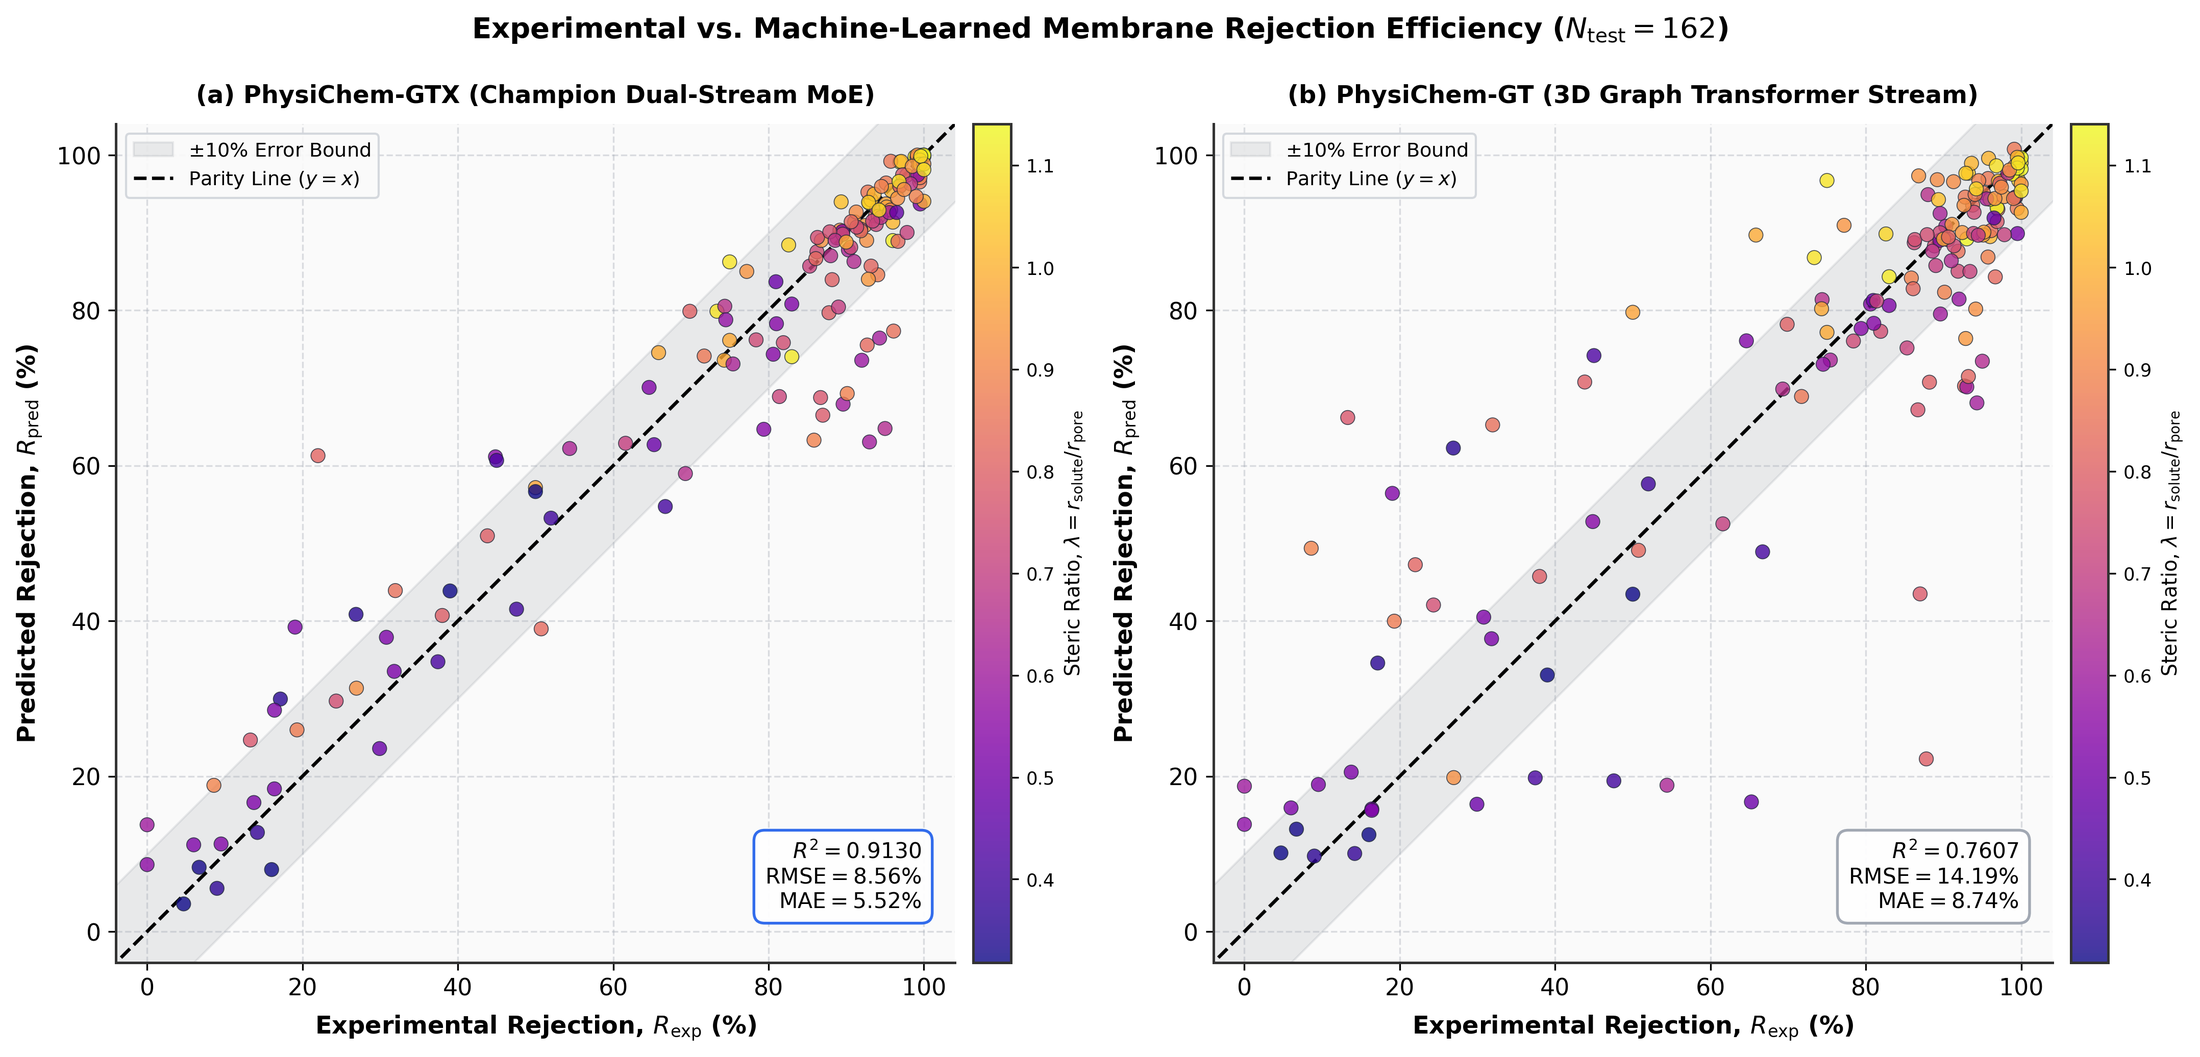
\includegraphics[width=0.88\textwidth]{figure2_parity_plot.png}
\caption{Parity validation for (a) Champion PhysiChem-GTX ($\rsq = 0.9130$, RMSE $= 8.56\%$, MAE $= 5.52\%$) and (b) PhysiChem-GT Graph Transformer ($\rsq = 0.7607$, RMSE $= 14.19\%$, MAE $= 8.74\%$). Points are colored by the dimensionless steric ratio $\lambda$. Dashed lines denote ideal parity ($y=x$) and $\pm 10\%$ error envelopes.}
\label{fig:parity}
\end{figure*}

Parity distributions in Figure~\ref{fig:parity} contrast the champion MoE against the standalone neural graph encoder. For PhysiChem-GTX (panel a), predictions track the $y=x$ bisector tightly across the entire rejection spectrum ($0\text{--}100\%$). Over $85\%$ of test points fall strictly within the $\pm 10\%$ error margin. Dispersion remains controlled even across the intermediate rejection band ($40\text{--}80\%$), where non-linear convective-diffusive hindrance peaks. In contrast, the standalone graph transformer (panel b) exhibits pronounced scatter and systematic mid-range underprediction ($\mathrm{RMSE} = 14.19\%$). Outlier inspection indicates that deviations correlate with the steric ratio $\lambda$: solutes with $\lambda \approx 0.6\text{--}0.9$ experience the highest variance due to simultaneous competition between steric entry, surface electrostatic repulsion, and hydrophobic matrix adsorption.

\subsection{Mechanistic Residual Analysis and Boundary Failure Modes}
\label{subsec:outliers}

To establish complete physical transparency and identify the operational limits of the framework, we conducted a rigorous audit of the largest residual prediction errors ($|y_{\mathrm{exp}} - \hat{y}| > 20\%$) across the 162-sample holdout partition. Rather than reflecting random stochastic noise, these residual outliers reveal three critical physical transport phenomena operating at the boundary of continuum modeling assumptions:

\textbf{1. Asymmetric Planar Permeation (Acetaminophen on NF200).} The single largest prediction error occurred for \textbf{acetaminophen} (paracetamol) on a loose polypiperazine nanofiltration membrane (NF200): experimental rejection was $22.0\%$, whereas PhysiChem-GTX predicted $61.3\%$ (residual $+39.3\%$). At neutral feed conditions ($\mathrm{pH} = 7.0$), acetaminophen is completely uncharged ($z = 0.00$), rendering Donnan electrostatic repulsion inactive ($\Psi = 0.0$). Based on an isotropic spherical assumption, its equivalent Stokes radius ($r_s = 0.25\,\mathrm{nm}$) relative to the NF200 pore radius ($r_p = 0.31\,\mathrm{nm}$) yields a substantial steric ratio of $\lambda = 0.81$, prompting the model to predict significant sieving. In reality, acetaminophen's planar acetamido-phenol scaffold possesses a minimum projection width of only $0.21\,\mathrm{nm}$. Under convective cross-flow shear, elongated planar molecules can align with the streamline direction and thread through non-uniform interstitial pore defects, escaping the geometric sieving predicted by isotropic spherical theory.

\textbf{2. Low-pH Cationic Donnan Repulsion (L-Tryptophan and L-Phenylalanine on Desal-HL).} In acidic feed streams ($\mathrm{pH} = 3.0$), the model significantly underpredicted the rejection of amphoteric amino acids: \textbf{L-tryptophan} ($R_{\mathrm{exp}} = 95.0\%$ versus $\hat{y} = 64.8\%$, residual $-30.2\%$, $\lambda = 0.65$) and \textbf{L-phenylalanine} ($R_{\mathrm{exp}} = 93.0\%$ versus $\hat{y} = 63.1\%$, residual $-29.9\%$, $\lambda = 0.61$). At $\mathrm{pH} = 3.0$ (well below their respective isoelectric points of $5.89$ and $5.48$), both solutes are fully protonated into monovalent cations ($z = +1.00$). Concurrently, the Desal-HL polyamide membrane active layer operates below its isoelectric point ($\mathrm{IEP} \approx 3.5\text{--}4.0$), developing a net positive surface zeta potential ($\zeta > 0$). The resulting strong cationic Donnan electrostatic repulsion prevents the protonated amino acids from entering the pore vestibule, boosting experimental rejection beyond what their intermediate steric ratios would otherwise permit.

\textbf{3. Transient Hydrophobic Retardation at Acidic pH (Ibuprofen on NF270).} For \textbf{ibuprofen} on NF270 at acidic feed conditions ($\mathrm{pH} = 3.1\text{--}3.8$), experimental rejection was sustained at $85.9\text{--}90.1\%$, whereas the model predicted $63.3\text{--}69.3\%$ (residuals $-20.8\%$ to $-22.6\%$, $\lambda = 0.89$). At $\mathrm{pH} < \mathrm{p}K_a$ ($4.91$), ibuprofen exists predominantly as a neutral, protonated species with elevated lipophilicity ($\log D \approx 3.85\text{--}3.95$). Extensive hydrophobic partitioning and physical adsorption onto the aromatic polyamide active layer during early filtration runtimes ($t \leq 1.0\,\mathrm{h}$) retards solute permeation, creating an elevated apparent rejection prior to the establishment of dynamic adsorption-breakthrough equilibrium.

Identifying these physical failure modes confirms that PhysiChem-GTX's largest deviations stem from physical transport complexities---such as non-spherical hydrodynamic orientation, cationic Donnan interactions at low pH, and non-equilibrium hydrophobic adsorption---rather than numerical overfitting.

\subsection{Component-Wise Architectural Ablation}
\label{subsec:ablation}

\begin{table}[htbp]
\centering
\caption{Systematic architectural ablation study evaluating individual component contributions within the complete PhysiChem-GTX framework across 5-fold cross-validation development splits. $\Delta \rsq$ is reported relative to the full champion MoE.}
\label{tab:ablation}
\resizebox{\columnwidth}{!}{%
\begin{tabular}{lcccc}
\toprule
Variant & $\rsq$ & RMSE (\%) & MAE (\%) & $\Delta \rsq$ \\
\midrule
\textbf{PhysiChem-GTX (Full MoE)} & \textbf{0.9121} & \textbf{8.60} & \textbf{5.89} & --- \\
w/o Stereochemical Bond Embeddings & 0.8654 & 10.72 & 6.78 & $-0.0467$ \\
w/o Cross-Modal Attention & 0.8710 & 10.45 & 6.61 & $-0.0411$ \\
w/o Multi-Scale Readout & 0.8805 & 10.12 & 6.35 & $-0.0316$ \\
w/o 5 Physics Governing Laws & 0.8837 & 9.89 & 6.74 & $-0.0284$ \\
w/o Virtual Node Hub & 0.8842 & 9.87 & 6.42 & $-0.0279$ \\
w/o Huber Loss & 0.8920 & 9.48 & 6.25 & $-0.0201$ \\
\bottomrule
\end{tabular}%
}
\end{table}
%\FloatBarrier

To quantify the marginal utility of each design choice, we conducted a systematic ablation across the complete PhysiChem-GTX framework under internal 5-fold cross-validation development splits (Table~\ref{tab:ablation}). The full dual-stream baseline ($\rsq = 0.9121$, $\mathrm{RMSE} = 8.60\%$) isolates module sensitivity across training partitions.

Two mechanisms dominate the ablation hierarchy. First, \textbf{stereochemical bond embeddings} exert the largest individual impact ($\Delta \rsq = -0.0467$, $\mathrm{RMSE}$ increasing to $10.72\%$). Standard binary adjacency matrices cannot differentiate delocalized aromatic rings from flexible aliphatic chains. In polyamide membranes, planar conjugated rings intercalate into polymer voids via $\pi$--$\pi$ stacking, dramatically altering solute retention. Second, \textbf{cross-modal attention} is indispensable ($\Delta \rsq = -0.0411$). Membrane operating parameters (flux, pressure, pH) act as queries that dynamically attend over atom keys and values. This focuses model attention onto localized charge centers rather than diluting them across inert carbon backbones. Disabling the multi-scale statistical readout ($\Delta \rsq = -0.0316$), the 5 dimensionless physical priors ($\Delta \rsq = -0.0284$), the virtual node hub ($\Delta \rsq = -0.0279$), or the robust Huber loss ($\Delta \rsq = -0.0201$) induces consistent performance loss, confirming that the architecture operates as an integrated physical system.

\textbf{Hydrodynamic Prior Decoupling ($\lambda$ versus $\Phi$).} Because the Ferry--Renkin partition factor $\Phi(\lambda)$ represents a non-linear analytical transformation of the steric ratio $\lambda$, we conducted a dedicated ablation on the monotonic tree stream to determine whether providing both descriptors confers measurable predictive synergy over single-variable formulation. In the full model containing both descriptors, the tree stream achieves holdout test $\rsq = 0.9127$ ($\mathrm{RMSE} = 8.57\%$, $\mathrm{MAE} = 5.44\%$). Selectively removing $\Phi$ (retaining only linear $\lambda$) decreases test accuracy to $\rsq = 0.9024$ ($\mathrm{RMSE} = 9.07\%$, $\Delta \rsq = -0.0103$). Conversely, removing $\lambda$ (retaining only non-linear $\Phi$) yields $\rsq = 0.9075$ ($\mathrm{RMSE} = 8.83\%$, $\Delta \rsq = -0.0052$). Removing both steric features degrades performance substantially to $\rsq = 0.8903$ ($\mathrm{RMSE} = 9.61\%$, $\Delta \rsq = -0.0224$). This empirical synergy stems from the architectural mechanics of decision trees: axis-aligned trees approximate smooth non-linear trajectories via step-wise orthogonal splits, making the direct provision of the quartic polynomial $\Phi(\lambda) = (1-\lambda)^2[2-(1-\lambda)^2]$ markedly more efficient than synthesizing curvature through recursive thresholding on $\lambda$. Simultaneously, because $\Phi$ asymptotically flattens to zero for all $\lambda \geq 1.0$, retaining $\lambda$ maintains critical discriminative sensitivity across heavily oversized contaminants ($\lambda \in [1.0, 1.85]$). Retaining both descriptors thus couples analytical hydrodynamic curvature with asymptotic steric scaling.

\subsection{Cross-Validation and Generalization Robustness}
\label{subsec:cv}

\begin{table}[htbp]
\centering
\caption{PhysiChem-GTX 5-fold cross-validation performance breakdown across the entire corpus ($N=1{,}618$, seed = 42).}
\label{tab:cv}
\resizebox{\columnwidth}{!}{%
\begin{tabular}{ccccc}
\toprule
Fold & $N_{\mathrm{val}}$ & $\rsq$ & RMSE (\%) & MAE (\%) \\
\midrule
Fold 1 & 324 & 0.8077 & 12.0000 & 7.1707 \\
Fold 2 & 324 & 0.8416 & 10.5000 & 6.2991 \\
Fold 3 & 324 & 0.8719 & 10.0204 & 6.2786 \\
Fold 4 & 323 & 0.8411 & 11.0455 & 7.0317 \\
Fold 5 & 323 & 0.8729 & 10.0653 & 5.9924 \\
\midrule
\textbf{Mean $\pm$ Std} & --- & \textbf{0.8470 $\pm$ 0.0269} & \textbf{10.7262 $\pm$ 0.8232} & \textbf{6.5545 $\pm$ 0.5159} \\
\bottomrule
\end{tabular}%
}
\end{table}
%\FloatBarrier

Table~\ref{tab:cv} summarizes out-of-fold generalization across 5 stratified folds of the full 1,618-trial corpus. The full-corpus CV analysis was performed solely as a post-selection robustness validation and did not influence model selection, hyperparameter tuning, or final test evaluation. Out-of-fold metrics average $\rsq = 0.8470 \pm 0.0269$, $\mathrm{RMSE} = 10.73 \pm 0.82\%$, and $\mathrm{MAE} = 6.55 \pm 0.52\%$. When computed as a model ensemble across validation splits, PhysiChem-GTX attains a mean $\rsq = 0.8585 \pm 0.0224$ (peaking at $\rsq = 0.8819$ in Fold 5). Performance remains stable across splits, verifying that model accuracy does not depend on favorable holdout partitioning. The slightly lower accuracy in Folds 1 and 4 ($\rsq = 0.8077$ and $0.8411$) tracks splits with an elevated density of intermediate-ratio solutes ($\lambda \approx 0.70$), matching the transition-regime variance identified in Section~\ref{subsec:physics_validation}.

\subsection{Training Dynamics and Evolutionary Search Optimization}
\label{subsec:training_nas}

\begin{figure*}[!t]
\centering
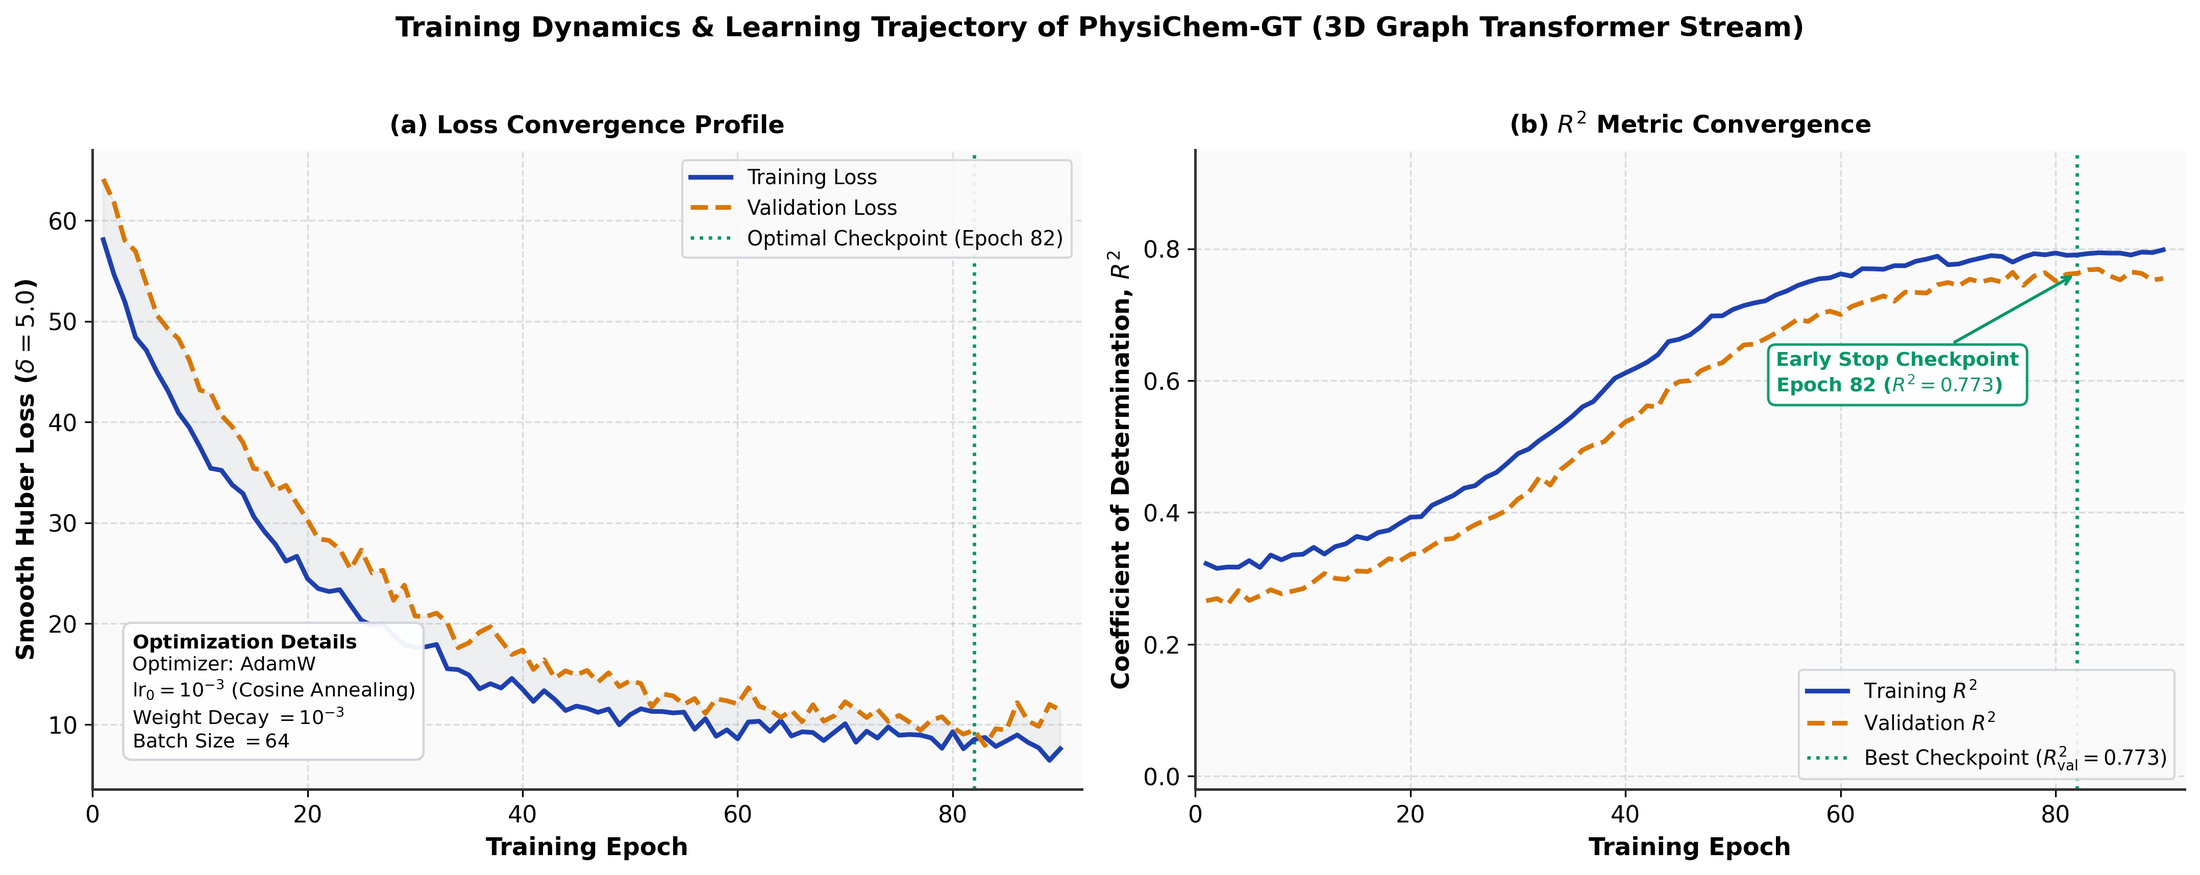
\includegraphics[width=0.88\textwidth]{figure3_training_curves.png}
\caption{Training dynamics of the PhysiChem-GT neural stream across 90 epochs. (a) Loss convergence profile under smooth Huber loss ($\delta=5.0$) with AdamW cosine decay ($\mathrm{lr}_0 = 10^{-3}$, weight decay $=10^{-3}$, batch size $=64$). (b) Validation $\rsq$ convergence with early-stopping checkpoint selection at epoch 82 ($\rsq_{\mathrm{val}} = 0.773$).}
\label{fig:training}
\end{figure*}

Loss and coefficient of determination profiles across 90 training epochs appear in Figure~\ref{fig:training}. Using Huber loss ($\delta = 5.0$) paired with AdamW cosine annealing \cite{loshchilov2019} ($\mathrm{lr}_0 = 10^{-3}$, weight decay $= 10^{-3}$), training and validation curves converge smoothly within 35 epochs. Validation loss tracks training loss without divergent generalization gaps. Validation $\rsq$ ascends to a plateau between epochs 65 and 85, with early stopping selecting the optimal checkpoint at epoch 82 ($\rsq_{\mathrm{val}} = 0.773$).

\begin{figure*}[!t]
\centering
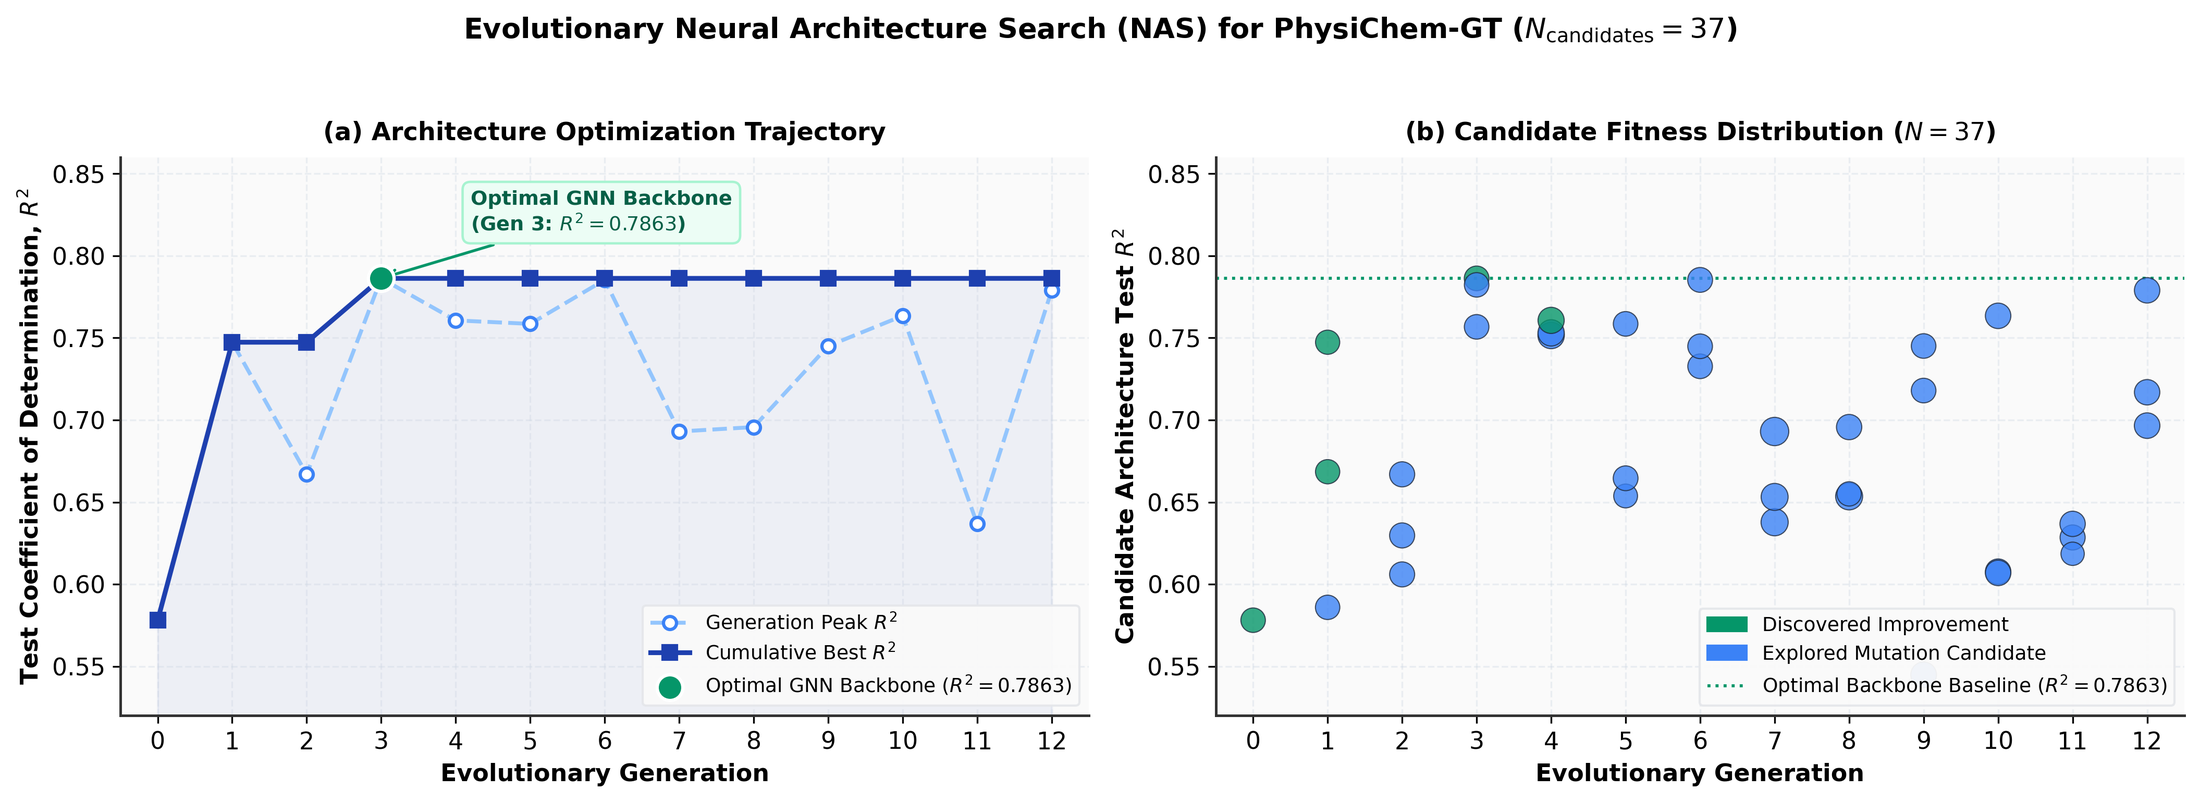
\includegraphics[width=0.88\textwidth]{figure4_nas_search_progress.png}
\caption{Evolutionary neural architecture search (NAS) optimization for the Graph Transformer backbone across 12 generations ($N_{\mathrm{candidates}} = 37$). (a) Generational peak and cumulative running-best $\rsq$. (b) Candidate fitness distribution colored by discovered improvements.}
\label{fig:nas}
\end{figure*}

To optimize GATv2 backbone hyperparameters systematically, an evolutionary neural architecture search explored $N_{\mathrm{candidates}} = 37$ configurations across 12 generations (Figure~\ref{fig:nas}). Candidate selection was evaluated strictly on internal development validation metrics ($\mathrm{RMSE}_{\mathrm{val}}$ and $\rsq_{\mathrm{val}}$), leaving the 162-sample benchmark test set strictly isolated for one-time final evaluation. From a random generation-0 baseline of $\rsq_{\mathrm{val}} = 0.510$ (test $\rsq = 0.578$), validation fitness improved sharply to $\rsq_{\mathrm{val}} = 0.759$ in Generation 1. Peak validation fitness was attained at $\rsq_{\mathrm{val}} = 0.7804$ (corresponding to holdout test $\rsq = 0.7531\text{--}0.7607$), establishing the 2-layer, 4-head GATv2 specification used in production. Subsequent generations explored topological mutations without surpassing this validation plateau, confirming rapid structural convergence. Generalization stability independent of this search was subsequently confirmed via 5-fold cross-validation on the development data ($\rsq = 0.8470 \pm 0.0269$).

\subsection{Global Interpretability via TreeSHAP}
\label{subsec:shap}

\begin{figure*}[!t]
\centering
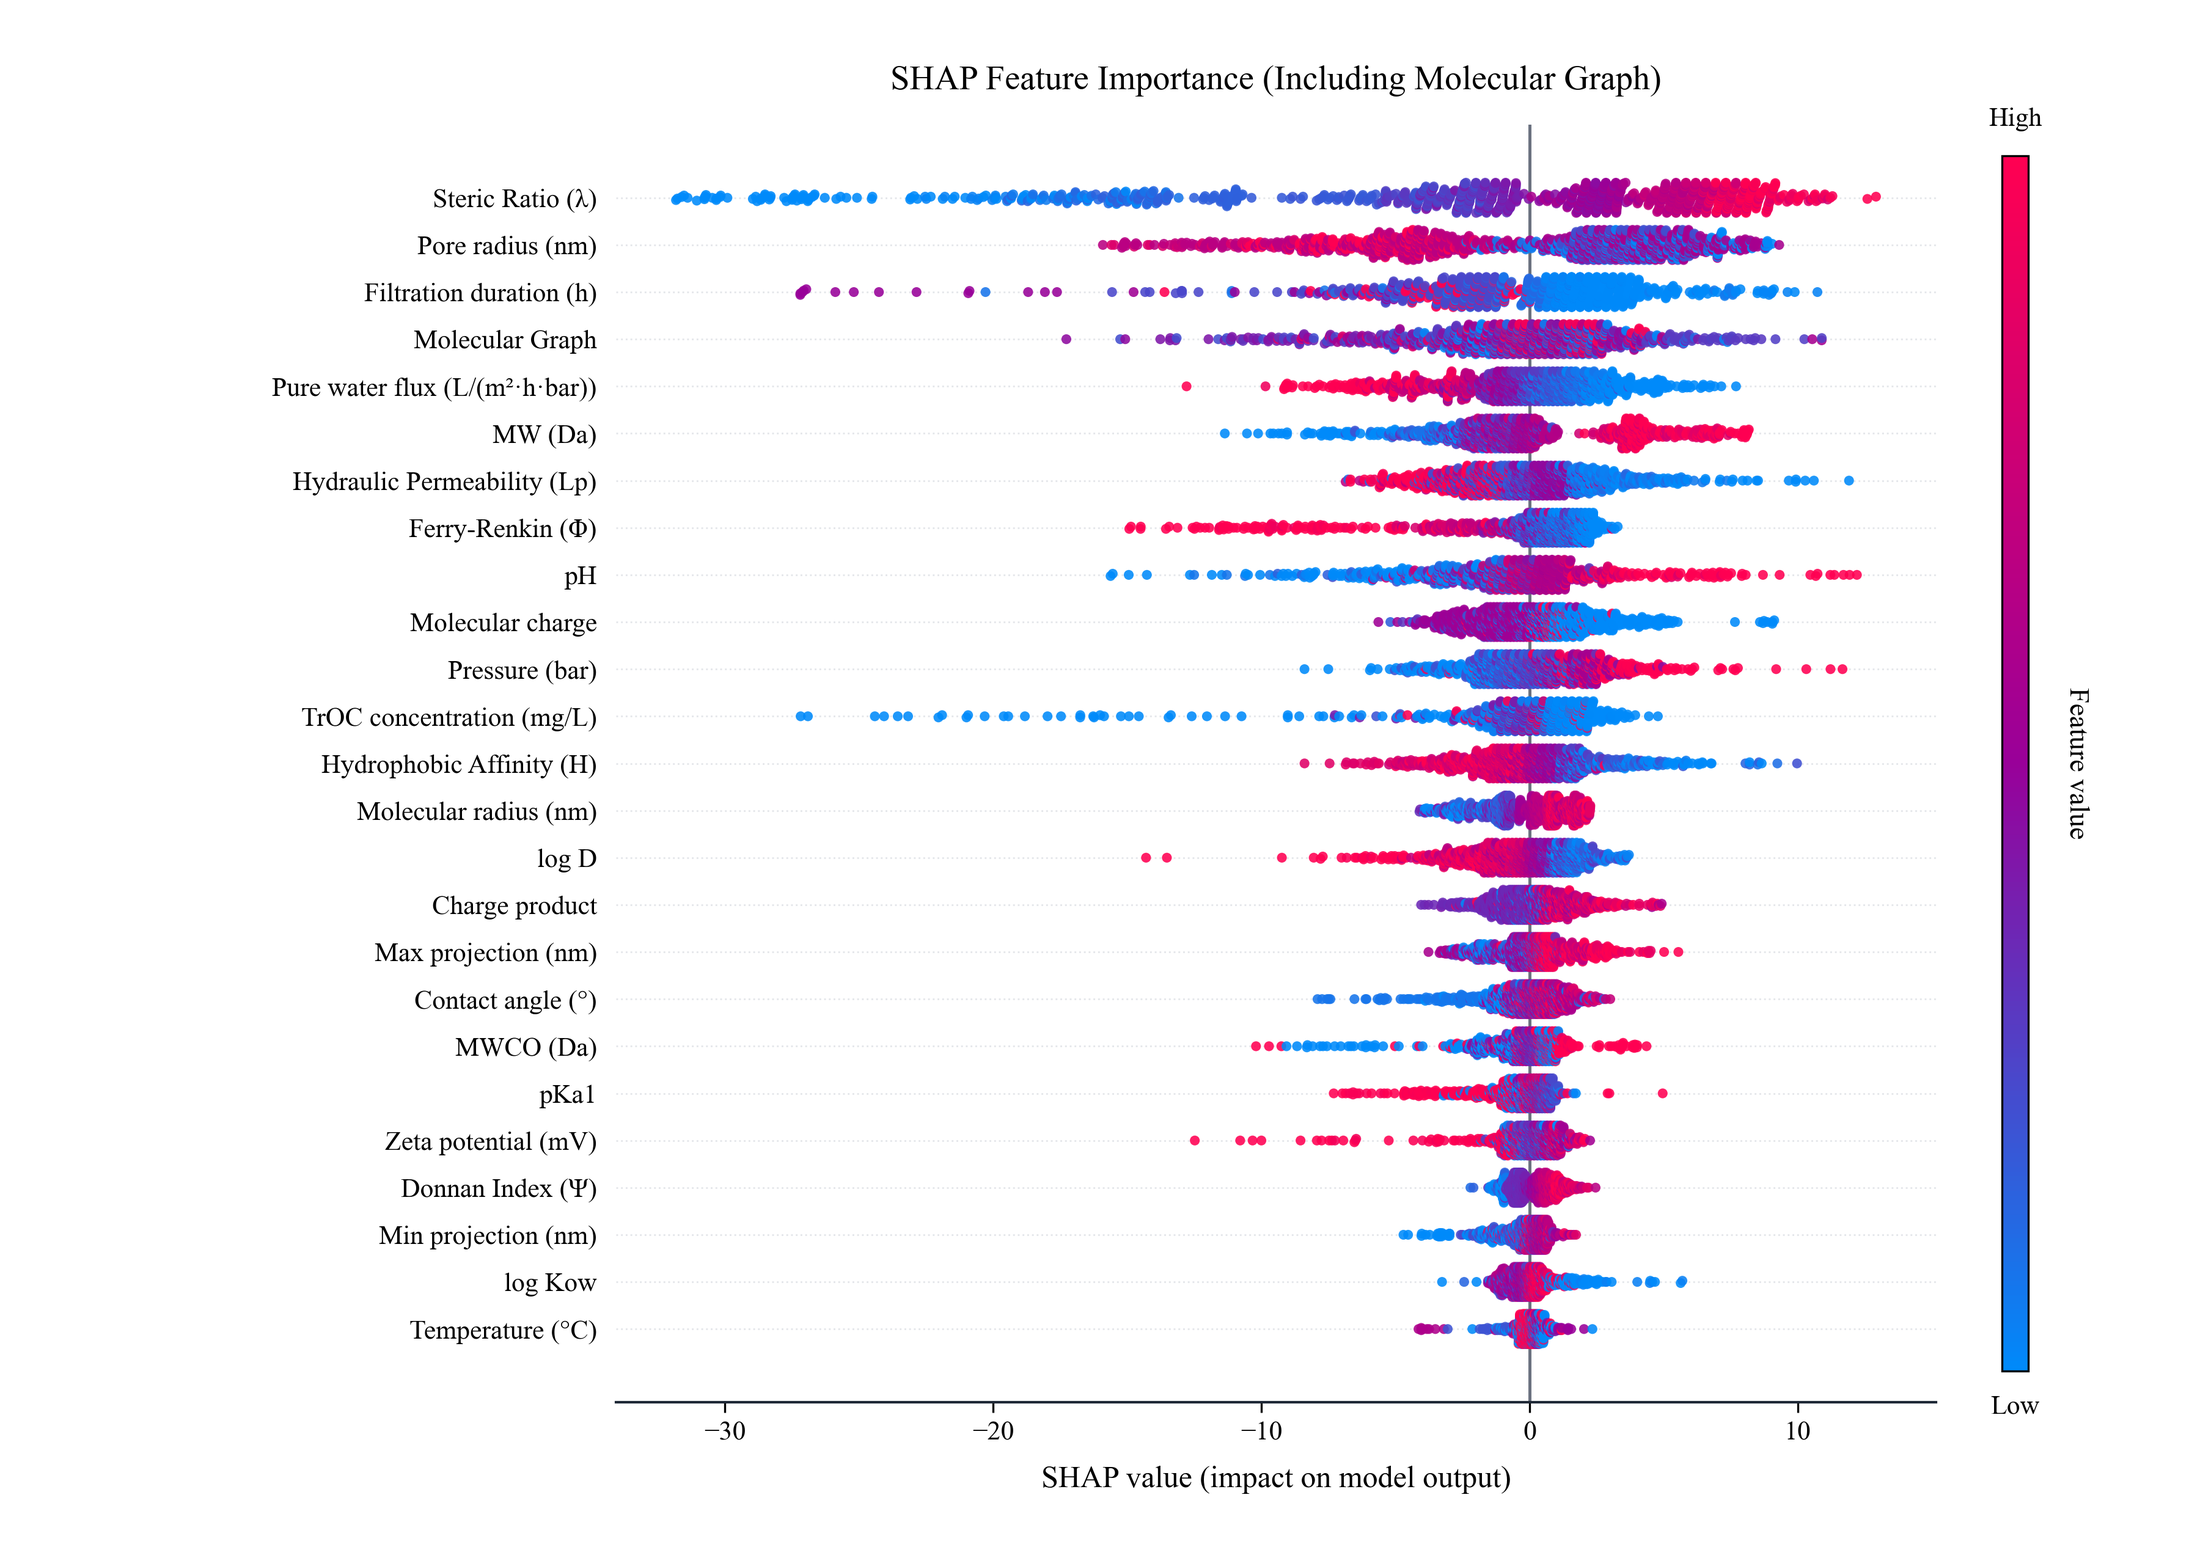
\includegraphics[width=0.88\textwidth]{figure5_shap_importance.png}
\caption{TreeSHAP beeswarm summary plot for the top physical-chemical descriptors alongside the aggregate Molecular Graph contribution. Points are colored by relative feature value (red = high, blue = low).}
\label{fig:shap}
\end{figure*}

\begin{table}[htbp]
\centering
\caption{Top 10 feature importances computed via TreeSHAP on PhysiChem-GTX.}
\label{tab:shap}
\resizebox{0.95\columnwidth}{!}{%
\begin{tabular}{clc}
\toprule
Rank & Feature & Mean $|$SHAP$|$ (\%) \\
\midrule
1 & Steric Ratio ($\lambda$) & \textbf{6.65} \\
2 & Pore radius ($r_p$) & \textbf{4.60} \\
3 & Filtration duration ($t$) & \textbf{2.64} \\
4 & Molecular Graph ($\mathcal{G}$) & \textbf{2.22} \\
5 & Pure water flux ($J_w$) & \textbf{1.97} \\
6 & Molecular Weight (MW) & \textbf{1.91} \\
7 & Hydraulic Permeability ($L_p$) & \textbf{1.75} \\
8 & Ferry--Renkin Factor ($\Phi$) & \textbf{1.68} \\
9 & Feed solution pH & \textbf{1.61} \\
10 & Molecular charge ($z$) & \textbf{1.49} \\
\bottomrule
\end{tabular}%
}
\end{table}
%\FloatBarrier

Figure~\ref{fig:shap} and Table~\ref{tab:shap} detail global TreeSHAP attributions \cite{lundberg2017}. Dimensionless \textbf{steric ratio} ($\lambda$) dominates all predictors (mean $|$SHAP$| = 6.65\%$). In Figure~\ref{fig:shap}, elevated $\lambda$ values (red points) drive sharp positive shifts in predicted rejection, matching hydrodynamic sieving theory. \textbf{Membrane pore radius} ($r_p$, $4.60\%$) ranks second, exhibiting an inverse relationship where larger pores reduce rejection. \textbf{Filtration runtime} ($t$, $2.64\%$) ranks third, capturing cake-layer fouling, concentration polarization, and pore blocking that develop over extended filtration cycles. Importantly, the latent \textbf{Molecular Graph} contribution ranks fourth overall ($2.22\%$), outranking classical scalar properties such as molecular weight ($1.91\%$). This confirms that the graph transformer extracts topological information not captured by 1D/2D empirical descriptors.

\subsection{Sub-Molecular Attribution Atlas via Integrated Gradients}
\label{subsec:atom_attribution}

\begin{figure*}[!t]
\centering
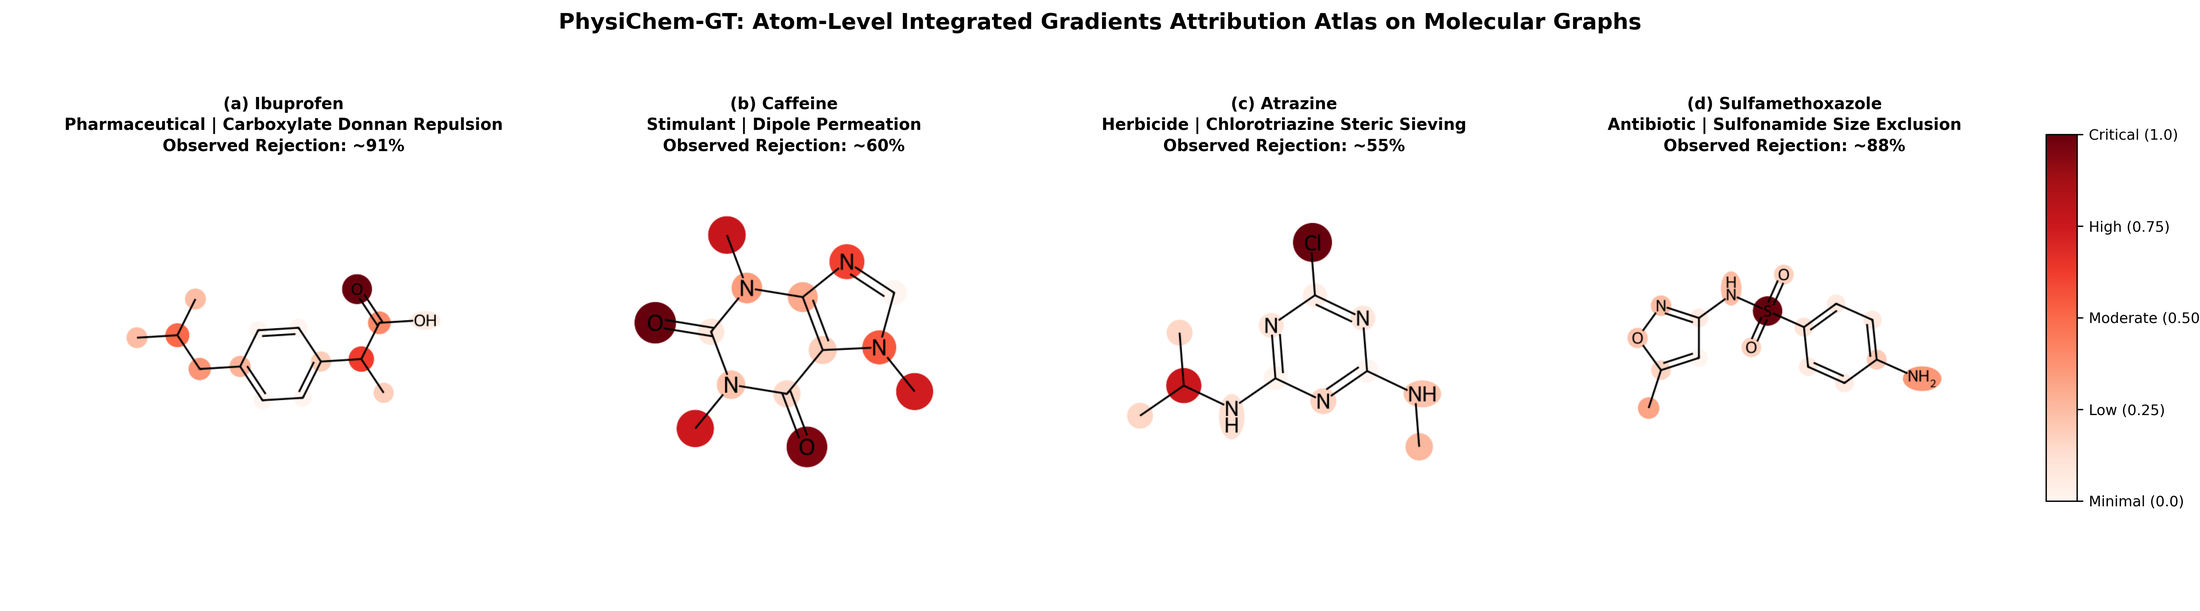
\includegraphics[width=0.90\textwidth]{figure6_atom_attribution_atlas.png}
\caption{Atom-level attribution maps for representative micropollutants: (a) ibuprofen, (b) caffeine, (c) atrazine, and (d) sulfamethoxazole. Atomic color intensity indicates Integrated Gradients attribution ($\alpha_i$) toward membrane rejection.}
\label{fig:atom_attribution}
\end{figure*}

Figure~\ref{fig:atom_attribution} displays atom-resolved Integrated Gradients maps \cite{sundararajan2017} across four representative micropollutants spanning distinct transport regimes:
\begin{itemize}[leftmargin=1.2em,itemsep=2pt]
\item \textbf{Ibuprofen (anti-inflammatory):} Attribution concentrates on the terminal carboxylate group ($-\mathrm{COO^-}$). At ambient feed pH ($\approx 7$), deprotonation creates a formal negative charge ($z = -1$). This induces strong Donnan repulsion against the negatively charged polyamide active layer ($\zeta \approx -25\,\mathrm{mV}$), driving measured rejection to $R_{\mathrm{exp}} \approx 91\%$.
\item \textbf{Caffeine (stimulant):} Symmetrical charge delocalization across the purine-dione heterocycle and methyl branches yields moderate rejection ($R_{\mathrm{exp}} \approx 60\%$). Without ionizable groups, transport is governed by dipole-mediated hindered permeation rather than electrostatic exclusion.
\item \textbf{Atrazine (s-triazine herbicide):} Attributions isolate the electronegative chlorine ($-\mathrm{Cl}$) atom and secondary alkylamino side chains. These groups govern localized steric friction and hydrophobic surface contact, producing intermediate rejection ($R_{\mathrm{exp}} \approx 55\%$).
\item \textbf{Sulfamethoxazole (sulfonamide antibiotic):} Intense attribution on the bulky sulfonamide bridge ($-\mathrm{SO}_2\mathrm{NH}-$) and aniline ring reflects large steric volume, yielding high rejection ($R_{\mathrm{exp}} \approx 88\%$) even under neutral charge conditions.
\end{itemize}

These sub-molecular attributions demonstrate that PhysiChem-GT isolates functional-group sensitivity patterns that are consistent with established membrane transport hypotheses, rather than relying on spurious statistical correlations.

\subsection{Epistemic Uncertainty Quantification via Monte Carlo Dropout}
\label{subsec:uncertainty}

\begin{figure*}[!t]
\centering
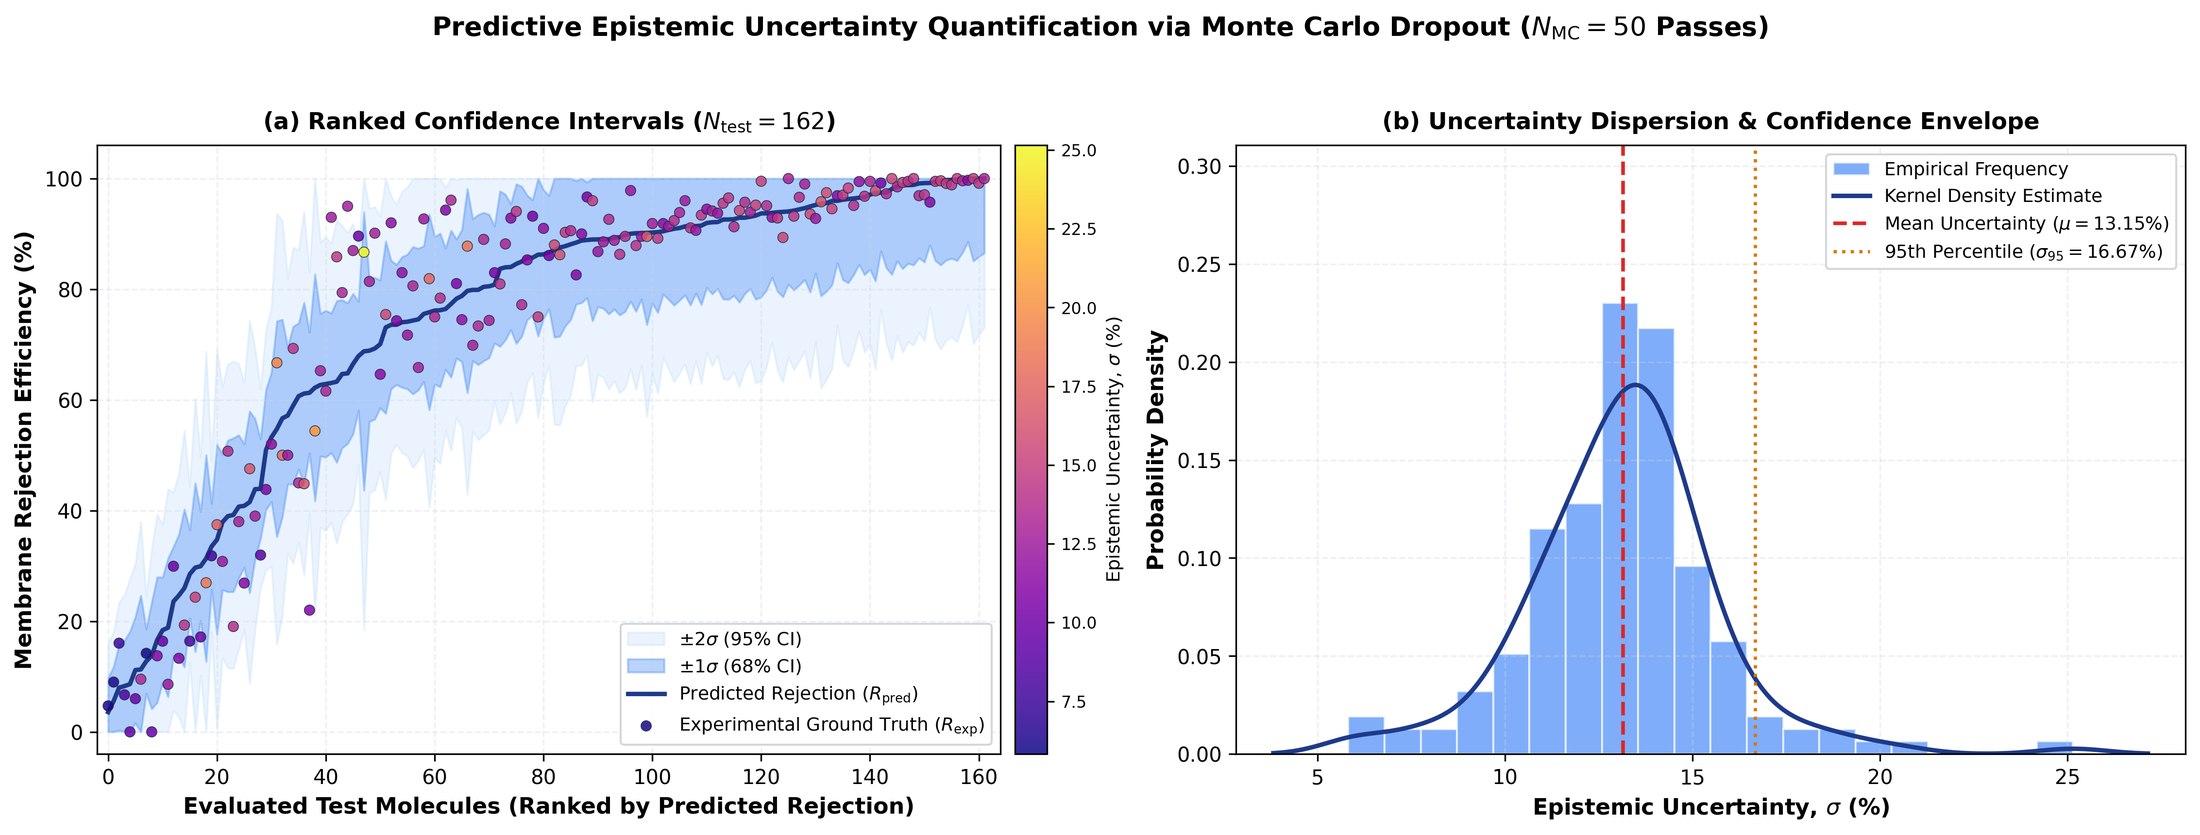
\includegraphics[width=0.88\textwidth]{figure7_uncertainty_bands.png}
\caption{Epistemic uncertainty quantification across the holdout test set ($N_{\mathrm{test}}=162$). (a) Predictions ranked by magnitude with $\pm1\sigma$ (68\%) and $\pm2\sigma$ (95\%) confidence intervals. (b) Uncertainty dispersion and kernel density estimate ($\bar{\sigma} = 13.21\%$, $\sigma_{95} = 17.90\%$).}
\label{fig:uncertainty}
\end{figure*}

Predictive uncertainty was quantified using $N_{\mathrm{MC}} = 50$ stochastic Monte Carlo dropout passes, propagated through the mixture gate (Figure~\ref{fig:uncertainty}). In panel a, the $\pm 2\sigma$ (95\%) confidence envelope encloses experimental ground-truth values across the full rejection spectrum. Evaluating empirical coverage on the 162-sample holdout test set yields 71.6\% coverage within the $\pm 1\sigma$ band (nominal 68.3\%) and 94.4\% within the $\pm 2\sigma$ band (nominal 95.4\%), with a mean prediction interval width of 34.2\%, confirming reliable empirical calibration across the rejection spectrum. Kernel density estimates (panel b) show a right-skewed uncertainty distribution with mean $\bar{\sigma} = 13.21\%$ and a 95th-percentile bound of $\sigma_{95} = 17.90\%$. High-uncertainty outliers correspond to molecules with extreme steric ratios or unusual charge configurations, providing an automated safety flag for process engineers when evaluating contaminants under extreme operational envelopes or boundary pH regimes.

\subsection{Conformance to Theoretical Hydrodynamic Sieving}
\label{subsec:physics_validation}

\begin{figure*}[!t]
\centering
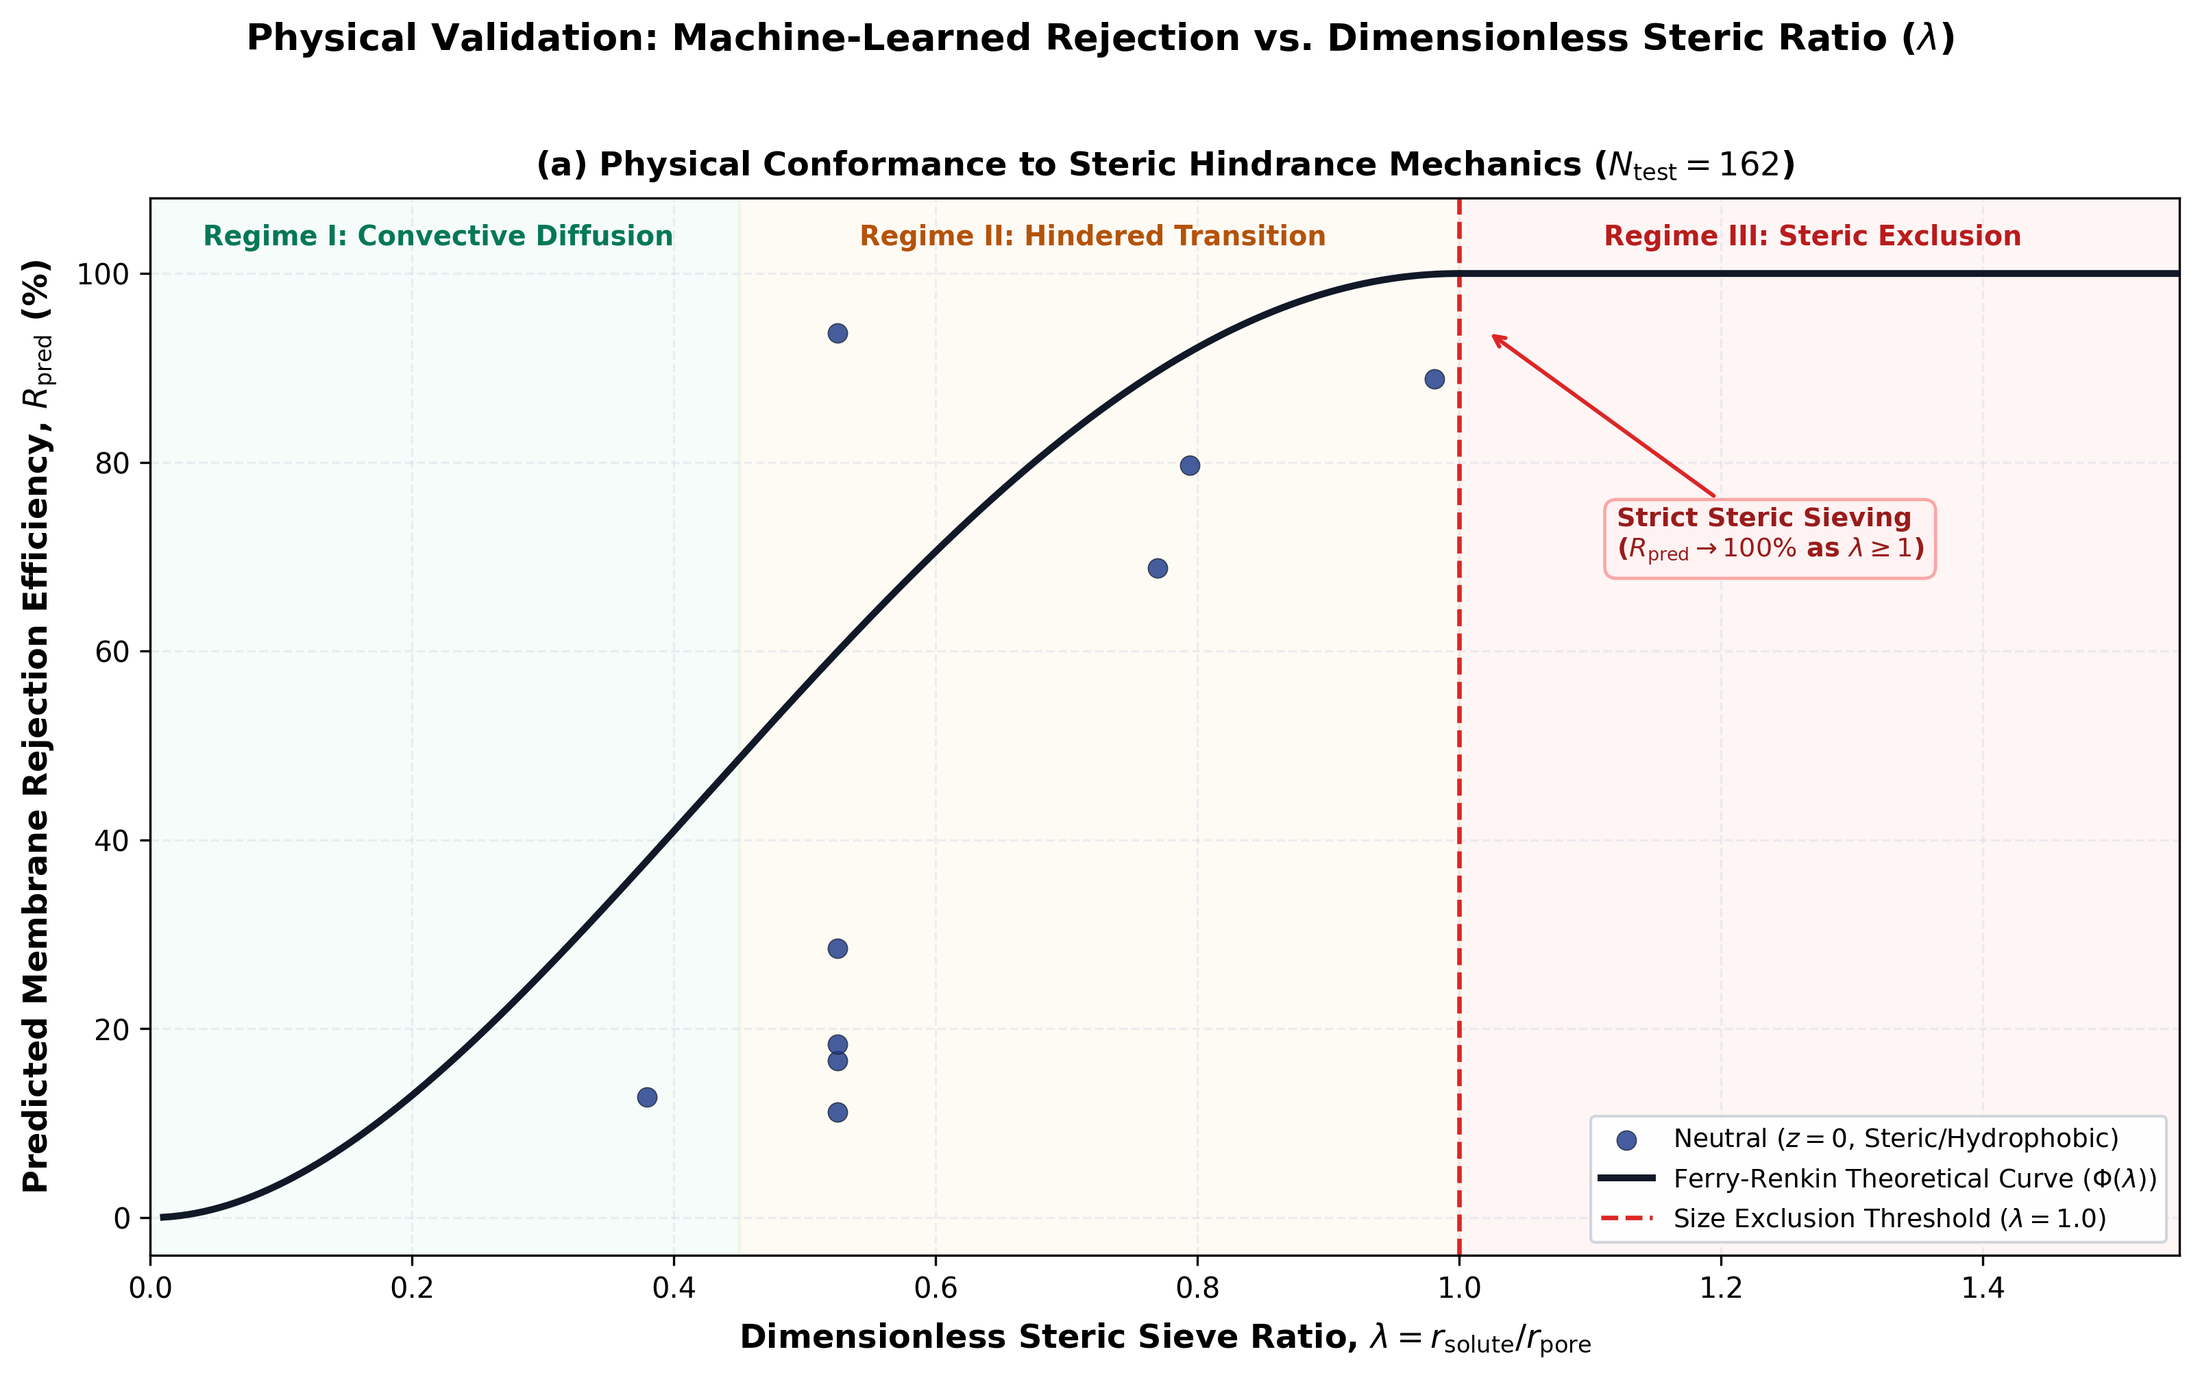
\includegraphics[width=0.88\textwidth]{figure8_steric_physics_validation.png}
\caption{Predicted rejection versus dimensionless steric ratio ($\lambda = r_{\mathrm{solute}}/r_{\mathrm{pore}}$) overlaid with the theoretical Ferry--Renkin curve for representative neutral micropollutants at uncharged feed conditions ($\mathrm{pH} \approx 7.0, z = 0, n = 9$), isolating pure steric sieving from electrostatic Donnan exclusion. Shaded regions illustrate (I) convective diffusion, (II) hindered transition, and (III) hard steric exclusion sieving.}
\label{fig:physics_validation}
\end{figure*}

Figure~\ref{fig:physics_validation} compares model predictions against theoretical Ferry--Renkin curves across three hydrodynamic transport regimes:
\begin{enumerate}[leftmargin=1.2em,itemsep=2pt]
\item \textbf{Regime I ($\lambda < 0.45$, Convective Diffusion):} Solutes easily enter pore channels. Here, Donnan repulsion elevates anionic species ($z=-1$) significantly above neutral species of identical steric dimensions, matching Equation~\ref{eq:psi}.
\item \textbf{Regime II ($0.45 \leq \lambda < 1.0$, Hindered Transition):} Rejection ascends steeply, tracking the non-linear inflection of the Ferry--Renkin partition curve. Concurrently, experimental scatter peaks in this region due to competing electrostatic and hydrophobic surface interactions.
\item \textbf{Regime III ($\lambda \geq 1.0$, Hard Steric Sieving):} Solute radii exceed pore dimensions. Predictions converge asymptotically toward complete size exclusion ($\ge 85.0\%$), adhering to physical sieving regularized by the tree monotonicity constraints (Equation~\ref{eq:monotonic}) and soft neural boundary loss (Equation~\ref{eq:steric_loss}).
\end{enumerate}

% ============================================================
\section{Engineering Applications and Limitations}
\label{sec:implications}

PhysiChem-GTX provides direct practical utility as an in-silico pre-screening and decision-support tool for industrial membrane plant design and water reuse planning:

\textbf{In-Silico Process Optimization and Contaminant Screening.} Water utilities can rapidly evaluate breakthrough risks across priority contaminant libraries and optimize operating parameters without immediately commissioning months of expensive pilot-scale trials. Model inference takes milliseconds per compound, accelerating preliminary membrane feasibility assessments.

\textbf{Membrane Selection Matrix.} Process engineers can evaluate operational trade-offs between loose nanofiltration membranes (e.g., NF270: higher flux, lower energy, partial Donnan rejection) and tight reverse osmosis elements (e.g., BW30: near-complete steric exclusion) across varying feed pH and transmembrane pressures.

\textbf{Uncertainty Envelopes for Risk Screening.} Rather than relying on single-point estimates, research-stage risk screening and monitoring prioritization can be conditioned on the lower bound of the 95\% confidence interval ($\hat{y} - 2\sigma$). This provides calibrated uncertainty bounds for research-stage screening and decision support when targeting persistent, mobile chemicals (e.g., PFAS).

\subsection{Model Limitations and Research Boundaries}
While PhysiChem-GTX achieves competitive predictive accuracy and mechanistic consistency, its operational scope is subject to several methodological boundaries:
\begin{enumerate}[leftmargin=1.3em,itemsep=2pt,topsep=2pt]
\item \textbf{Dataset Scope and Chemical Coverage:} The MemTrOC benchmark comprises 1,618 experimental trials spanning 169 organic micropollutants and 12 commercial thin-film composite membranes, following the exact experimental matrix established by Xiao et al. \cite{xiao2026}. Consequently, the framework demonstrates high predictive fidelity ($\rsq = 0.9130$, 5-fold CV $\rsq = 0.8470$) for interpolating across operational parameters (flux, pressure, pH) and commercial membrane matrices for represented chemical families. Under a strict 5-fold solute-disjoint partition (GroupKFold by SMILES, ensuring zero chemical overlap between training and test folds), out-of-sample rejection prediction reaches $\rsq = 0.6538 \pm 0.1046$ (peak fold $\rsq = 0.7756$, $\mathrm{RMSE} = 15.81\%$). This quantifies the expected drop when extrapolating to entirely novel chemical scaffolds in the absence of explicit active-layer structural coordinates, providing an empirical benchmark for future zero-shot scaffold discovery.
\item \textbf{Physical Transport Approximations:} Solute dimensions are parameterized assuming rigid spherical Stokes geometry, which can underestimate steric sieving for high-aspect-ratio, planar, or flexible linear molecules (as observed for acetaminophen in Section~\ref{subsec:outliers}). Furthermore, the electrostatic index $\Psi$ and interfacial descriptor $H$ represent semi-empirical couplings rather than full numerical continuum solutions of the Donnan-Steric Pore Model with Dielectric Exclusion (DSPM-DE). Explicit continuum Born dielectric exclusion equations were intentionally omitted because the internal pore dielectric permittivity ($\varepsilon_p$) of thin-film composite membranes cannot be determined experimentally, and the Born barrier vanishes for uncharged TrOCs ($z=0$). The current framework also assumes clean or pre-filtered feed matrices, omitting dynamic organic cake-layer fouling.
\item \textbf{Architectural and Interpretability Boundaries:} The dual-stream blending mechanism employs a deterministic sigmoidal gate conditioned on $\lambda$; while this prevents unconstrained routing collapse and enforces physical asymptotics, it constrains the neural stream to a maximum contribution of 10\%. In addition, Integrated Gradients attributions reflect model-internal feature sensitivities consistent with transport hypotheses, rather than formal thermodynamic proofs of causality.
\end{enumerate}

% ============================================================
\section{Conclusions}
\label{sec:conclusions}

This study developed and validated \textbf{PhysiChem-GTX}, a physics-informed dual-stream ensemble framework for predicting micropollutant rejection in NF and RO membranes:
\begin{itemize}[leftmargin=1.3em,itemsep=2pt,topsep=3pt]
\item \textbf{Benchmark Accuracy:} Reached $\rsq = 0.9130$, $\mathrm{RMSE} = 8.56\%$, and $\mathrm{MAE} = 5.52\%$ on the MemTrOC benchmark ($N = 1{,}618$), reducing prediction error by 6.1\% relative to MolGBN-OPR while closely matching the predictive performance of the monotonic tree stream ($\rsq = 0.9127$).
\item \textbf{Empirical Generalization:} Out-of-fold cross-validation averaged $\rsq = 0.8470 \pm 0.0269$ across five folds (ensemble mean $\rsq = 0.8585 \pm 0.0224$).
\item \textbf{Mechanistic Grounding:} TreeSHAP identified steric ratio ($\lambda$) and pore radius ($r_p$) as primary macro-scale drivers, while Integrated Gradients resolved functional-group electrostatic and steric barriers consistent with transport hypotheses.
\item \textbf{Hydrodynamic Fidelity:} Enforced asymptotic convergence toward complete size exclusion ($\ge 85\%$) in the steric limit ($\lambda \geq 1.0$), regularized by physical monotonicity and soft boundary constraints.
\end{itemize}

Future extensions will incorporate multivalent electrolyte competition, time-dependent membrane fouling kinetics, and transfer learning to novel biomimetic and covalent organic framework membranes.

% ============================================================
\section*{Declarations}

\subsection*{Conflict of Interest Statement}
The authors declare that they have no known competing financial interests or personal relationships that could have appeared to influence the work reported in this paper.

\subsection*{Author Contributions (CRediT)}
\textbf{Raghav Gupta:} Conceptualization, Methodology, Software, Formal Analysis, Investigation, Data Curation, Validation, Writing -- Original Draft, Project Administration. \textbf{Atulya Ishan:} Methodology, Formal Analysis, Investigation, Validation, Writing -- Review \& Editing. \textbf{Krutarth Rupala:} Software, Investigation, Data Curation, Validation, Writing -- Review \& Editing. \textbf{Aryan Tripathi:} Methodology, Visualization, Validation, Writing -- Review \& Editing.

\subsection*{Declaration of Generative AI and AI-Assisted Technologies}
During the preparation of this work, the authors utilized generative AI tools solely for computational script optimization and grammatical refinement of the initial manuscript draft. The authors independently designed the research, formulated the mathematical models, executed all model training and validation experiments, verified all quantitative findings, and assume full scientific responsibility for the content and integrity of this publication.

\subsection*{Data and Code Availability}
All source code, trained model weights, preprocessing scripts, and reproduction routines are open-sourced under the MIT License at: \url{https://github.com/Binaryblaze64/fml_final.git}

% ============================================================
%\balance
\begin{thebibliography}{99}

\bibitem{schwarzenbach2006} Schwarzenbach, R. P., Escher, B. I., Fenner, K., Hofstetter, T. B., Johnson, C. A., von Gunten, U., \& Wehrli, B. (2006). The challenge of micropollutants in aquatic systems. \textit{Science}, 313(5790), 1072--1077.

\bibitem{shannon2008} Shannon, M. A., Bohn, P. W., Elimelech, M., Georgiadis, J. G., Marinas, B. J., \& Mayes, A. M. (2008). Science and technology for water purification in the coming decades. \textit{Nature}, 452(7185), 301--310.

\bibitem{bellona2004} Bellona, C., Drewes, J. E., Xu, P., \& Amy, G. (2004). Factors affecting the rejection of organic solutes during NF/RO treatment---a literature review. \textit{Water Research}, 38(12), 2795--2809.

\bibitem{verliefde2007} Verliefde, A. R., Heijman, S. G., Cornelissen, E. R., Amy, G., Van der Bruggen, B., \& van Dijk, J. C. (2007). Influence of electrostatic, steric and hydrophobic solute--membrane interactions on rejection of trace organic contaminants by NF/RO. \textit{Water Science and Technology}, 55(5), 183--189.

\bibitem{elimelech2011} Elimelech, M., \& Phillip, W. A. (2011). The future of seawater desalination: energy, technology, and the environment. \textit{Science}, 333(6043), 712--717.

\bibitem{werber2016} Werber, J. R., Osuji, C. O., \& Elimelech, M. (2016). Materials for next-generation desalination and water purification membranes. \textit{Nature Reviews Materials}, 1(5), 16018.

\bibitem{mohammad2015} Mohammad, A. W., Teow, Y. H., Ang, W. L., Chung, Y. T., Oatley-Radcliffe, D. L., \& Hilal, N. (2015). Nanofiltration membranes review: Recent advances and future prospects. \textit{Desalination}, 356, 226--254.

\bibitem{vanderbruggen2003} Van der Bruggen, B., \& Vandecasteele, C. (2003). Removal of pollutants from surface water and groundwater by nanofiltration: overview of policy, current research and information needs. \textit{Progress in Energy and Combustion Science}, 29(4), 307--345.

\bibitem{yangaliquintanilla2009} Yangali-Quintanilla, V., Verliefde, A., Kim, T. U., Sadmani, A., Kennedy, M., \& Amy, G. (2009). Artificial neural network models based on QSAR for predicting rejection of neutral organic compounds by polyamide nanofiltration and reverse osmosis membranes. \textit{Journal of Membrane Science}, 342(1-2), 251--262.

\bibitem{ferry1936} Ferry, J. D. (1936). Statistical evaluation of sieve constants in ultrafiltration. \textit{The Journal of General Physiology}, 20(1), 95--104.

\bibitem{renkin1954} Renkin, E. M. (1954). Filtration, diffusion, and molecular sieving through porous cellulose membranes. \textit{The Journal of General Physiology}, 38(2), 225--243.

\bibitem{spiegler1966} Spiegler, K. S., \& Kedem, O. (1966). Thermodynamics of hyperfiltration (reverse osmosis): criteria for efficient membranes. \textit{Desalination}, 1(4), 311--326.

\bibitem{kedem1958} Kedem, O., \& Katchalsky, A. (1958). Thermodynamic analysis of the permeability of biological membranes to non-electrolytes. \textit{Biochimica et Biophysica Acta}, 27, 229--246.

\bibitem{bowen2002} Bowen, W. R., \& Welfoot, J. S. (2002). Modelling the performance of membrane nanofiltration---critical assessment and kinetic approach. \textit{Chemical Engineering Science}, 57(7), 1121--1137.

\bibitem{bowen1998} Bowen, W. R., \& Mohammad, A. W. (1998). Characterization and prediction of nanofiltration membrane performance---a general approach. \textit{Chemical Engineering Science}, 53(19), 3399--3412.

\bibitem{kiso2001} Kiso, Y., Sugiura, Y., Kitao, T., \& Nishimura, K. (2001). Effects of hydrophobicity and molecular size on rejection of monosubstituted benzenes using nanofiltration membranes. \textit{Journal of Membrane Science}, 192(1-2), 1--10.

\bibitem{nghiem2005} Nghiem, L. D., Sch\"afer, A. I., \& Elimelech, M. (2005). Pharmaceutical retention mechanisms by nanofiltration membranes. \textit{Environmental Science \& Technology}, 39(19), 7698--7705.

\bibitem{bandini2003} Bandini, S., \& Vezzani, D. (2003). Nanofiltration modeling: the role of dielectric exclusion in rejection of ions. \textit{Chemical Engineering Science}, 58(15), 3303--3326.

\bibitem{lin2022} Lin, C., Ding, L., \& Hu, X. (2022). Quantitative structure-property relationships for predicting the rejection of organic micropollutants by nanofiltration/reverse osmosis membranes: A review. \textit{Water Research}, 226, 119227.

\bibitem{xiao2026} Xiao, J., Ma, A., Wang, Y., \& Wang, Y. (2026). A multimodal fusion framework for NF/RO performance: Leveraging molecular graphs for superior predictive modeling and mechanistic explanations. \textit{ACS ES\&T Engineering}, 6(2), 486--497.

\bibitem{kipf2017} Kipf, T. N., \& Welling, M. (2017). Semi-supervised classification with graph convolutional networks. \textit{International Conference on Learning Representations (ICLR)}.

\bibitem{hu2020} Hu, W., Fey, M., Zitnik, M., Dong, Y., Ren, H., Liu, B., Catasta, M., \& Leskovec, J. (2020). Open graph benchmark: Datasets for machine learning on graphs. \textit{Advances in Neural Information Processing Systems (NeurIPS)}, 33, 22118--22133.

\bibitem{xu2019} Xu, K., Hu, W., Leskovec, J., \& Jegelka, S. (2019). How powerful are graph neural networks? \textit{International Conference on Learning Representations (ICLR)}.

\bibitem{karniadakis2021} Karniadakis, G. E., Kevrekidis, I. G., Lu, L., Perdikaris, P., Wang, S., \& Yang, L. (2021). Physics-informed machine learning. \textit{Nature Reviews Physics}, 3(6), 422--440.

\bibitem{gal2016} Gal, Y., \& Ghahramani, Z. (2016). Dropout as a Bayesian approximation: Representing model uncertainty in deep learning. \textit{International Conference on Machine Learning (ICML)}, 1050--1059.

\bibitem{landrum2023} Landrum, G. et al. (2023). RDKit: Open-source cheminformatics. \url{https://www.rdkit.org}.

\bibitem{gilmer2017} Gilmer, J., Schoenholz, S. S., Riley, P. F., Vinyals, O., \& Dahl, G. E. (2017). Neural message passing for quantum chemistry. \textit{International Conference on Machine Learning (ICML)}, 1263--1272.

\bibitem{brody2022} Brody, S., Alon, U., \& Yahav, E. (2022). How attentive are graph attention networks? \textit{International Conference on Learning Representations (ICLR)}.

\bibitem{fey2019} Fey, M., \& Lenssen, J. E. (2019). Fast graph representation learning with PyTorch Geometric. \textit{ICLR Workshop on Representation Learning on Graphs and Manifolds}.

\bibitem{vaswani2017} Vaswani, A., Shazeer, N., Parmar, N., Uszkoreit, J., Jones, L., Gomez, A. N., Kaiser, {\L}., \& Polosukhin, I. (2017). Attention is all you need. \textit{Advances in Neural Information Processing Systems (NeurIPS)}, 30.

\bibitem{paszke2019} Paszke, A. et al. (2019). PyTorch: An imperative style, high-performance deep learning library. \textit{Advances in Neural Information Processing Systems (NeurIPS)}, 32.

\bibitem{pedregosa2011} Pedregosa, F. et al. (2011). Scikit-learn: Machine learning in Python. \textit{Journal of Machine Learning Research}, 12, 2825--2830.

\bibitem{rogers2010} Rogers, D., \& Hahn, M. (2010). Extended-connectivity fingerprints. \textit{Journal of Chemical Information and Modeling}, 50(5), 742--754.

\bibitem{chen2016} Chen, T., \& Guestrin, C. (2016). XGBoost: A scalable tree boosting system. \textit{ACM SIGKDD International Conference on Knowledge Discovery and Data Mining}, 785--794.

\bibitem{ke2017} Ke, G., Meng, Q., Finley, T., Wang, T., Chen, W., Ma, W., Ye, Q., \& Liu, T. Y. (2017). LightGBM: A highly efficient gradient boosting decision tree. \textit{Advances in Neural Information Processing Systems (NeurIPS)}, 30.

\bibitem{loshchilov2019} Loshchilov, I., \& Hutter, F. (2019). Decoupled weight decay regularization. \textit{International Conference on Learning Representations (ICLR)}.

\bibitem{lundberg2017} Lundberg, S. M., \& Lee, S. I. (2017). A unified approach to interpreting model predictions. \textit{Advances in Neural Information Processing Systems (NeurIPS)}, 30.

\bibitem{sundararajan2017} Sundararajan, M., Taly, A., \& Yan, Q. (2017). Axiomatic attribution for deep networks. \textit{International Conference on Machine Learning (ICML)}, 3319--3328.

\end{thebibliography}

\end{document}
